
\documentclass[]{article}
\usepackage[margin=1in]{geometry}

%% PACKAGES
%\usepackage{hyperref}
\usepackage{graphicx}
\usepackage[usenames,dvipsnames]{xcolor}
\usepackage{listings,amsmath}
\usepackage{microtype,todonotes}
\usepackage[strings]{underscore}
\usepackage{fancyvrb}
\VerbatimFootnotes

%% GRAPHICS RELATED
\usepackage[outdir=./tmp/]{epstopdf}
\graphicspath{{../images/}{./tmp}}
\DeclareGraphicsExtensions{.eps, .pdf, .jpeg, .png}

%% BIBLIOGRAPHY
\bibliographystyle{ieeetr}

%% CPATION SETUP
\usepackage{caption}
\usepackage{subcaption}
\usepackage{subfig}
\captionsetup{belowskip=12pt,aboveskip=4pt}

%% EQUATIONS
\numberwithin{equation}{section}

%% LISTINGS
\lstset{ %
    language=C++,
    basicstyle=\footnotesize\ttfamily,
    numbers=left,
    numberstyle=\tiny\color{gray},
    stepnumber=2,
    numbersep=5pt,
    backgroundcolor=\color{white},
    showspaces=false,
    showstringspaces=false,
    showtabs=false,
    frame=single,
    rulecolor=\color{black},
    tabsize=2,
    breaklines=true,
    breakatwhitespace=false,
    title=\lstname,
    keywordstyle=\color{blue},
    commentstyle=\color{OliveGreen},
    stringstyle=\color{orange}
}
\DeclareCaptionFont{white}{\color{white}}
\DeclareCaptionFormat{listing}{\colorbox[cmyk]{0.43, 0.35, 0.35, 0.01}{\parbox{\dimexpr\textwidth-2\fboxsep\relax}{#1#2#3}}}
\captionsetup[lstlisting]{format=listing,labelfont=white,textfont=white,singlelinecheck=false,margin=0pt,font={bf,footnotesize}}
\lstnewenvironment{code}[1][]%
{ \noindent\minipage{\linewidth}
	\lstset{#1}
}
{\endminipage}

%% USER COMMANDS
\newcommand{\iso}[2]{${}^{#2}${#1}}
\newcommand{\figurewidth}{\textwidth}

\title{Energy Deposition in Polymers}
\author{Matthew J. Urffer}
\date{\today}

\begin{document}

% Cover Page
\maketitle

% To Do List
\listoftodos

% Tables of Contents, Figures, Tables
\tableofcontents
\listoffigures
\listoftables

% !TEX TS-program = pdflatex
% !TEX encoding = UTF-8 Unicode

% Matthew Urffer Master Thesis
% INTRODUCTORY MATERIAL 

\section{Introduction}

\subsection{Radiation Portal Monitors}

%%%%%%%%%%%%%%%%%%%%%%%%%%%%%%%%%%%%%%%%%%%%%%%%%%%%%%%%%%%%%%%%%%%%%%%%%%%%%%%
\begin{frame}{U.S. Border Traffic}
\begin{columns}[onlytextwidth]
\begin{column} {0.45\textwidth}
 
  \begin{itemize}
  \item Every day 932,456 people cross into the U.S. \cite{cpb_typical_2012}
    \begin{itemize}
    	\item 259,191 by air
	\item 48,073 by sea
	\item 621,874 by land
    \end{itemize}
  \item 64,483 truck, rail and sea containers \cite{cpb_typical_2012}
 \item 253,821 privately-owned vehicles \cite{cpb_typical_2012}
  \end{itemize}
\end{column}
\begin{column}{0.45\textwidth}
\centering
\begin{figure}
		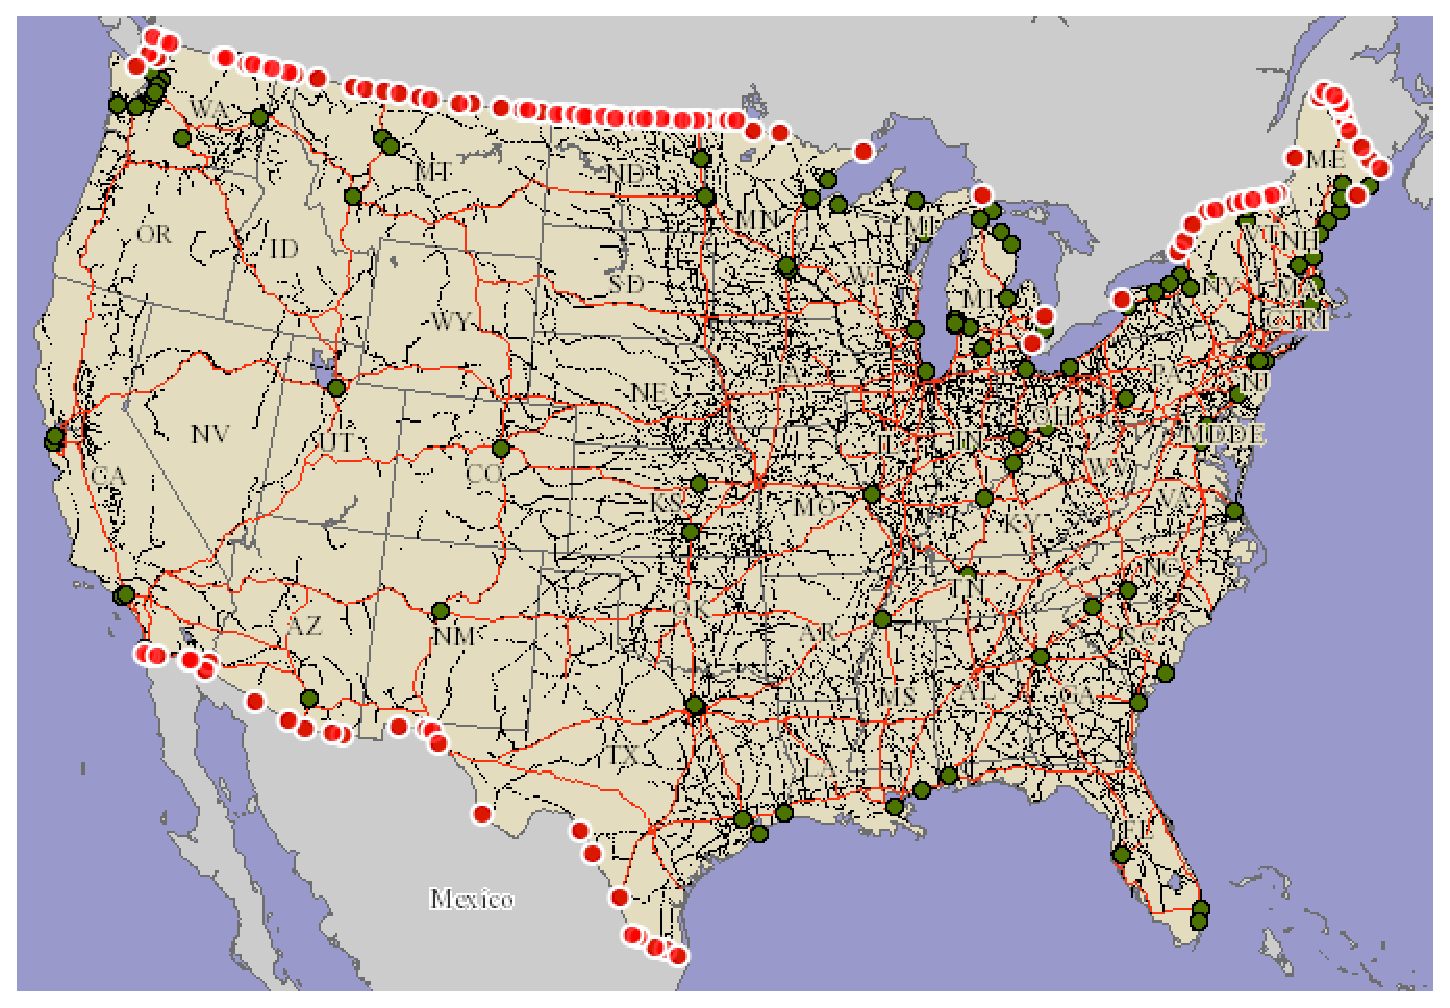
\includegraphics[width=\textwidth]{images/PortalEntryMap.eps}
		\label{fig:PortalEntryMap}
	\caption{Portal Entry Points into the U.S.}
\end{figure}
\end{column}
\end{columns}
\end{frame}

%%%%%%%%%%%%%%%%%%%%%%%%%%%%%%%%%%%%%%%%%%%%%%%%%%%%%%%%%%%%%%%%%%%%%%%%%%%%%%%
\begin{frame}{Radiation Portal Monitors}
\begin{columns}[onlytextwidth]
	\begin{column} {0.45\textwidth}
  	\begin{itemize}
  		\item Radiation portal monitors (RPMs) are passive radiation detectors
  		\item {
  			 RPMs are currently   ${}^3$He based detectors
  			\center
    		${}^3He +n \to p +{}^3H$
    	}
  		\item 
  			Shortage of ${}^3$He, so alternatives are being explored
  		\end{itemize}
	\end{column}
	\begin{column}{0.5\textwidth}
		\centering
		\begin{figure}
			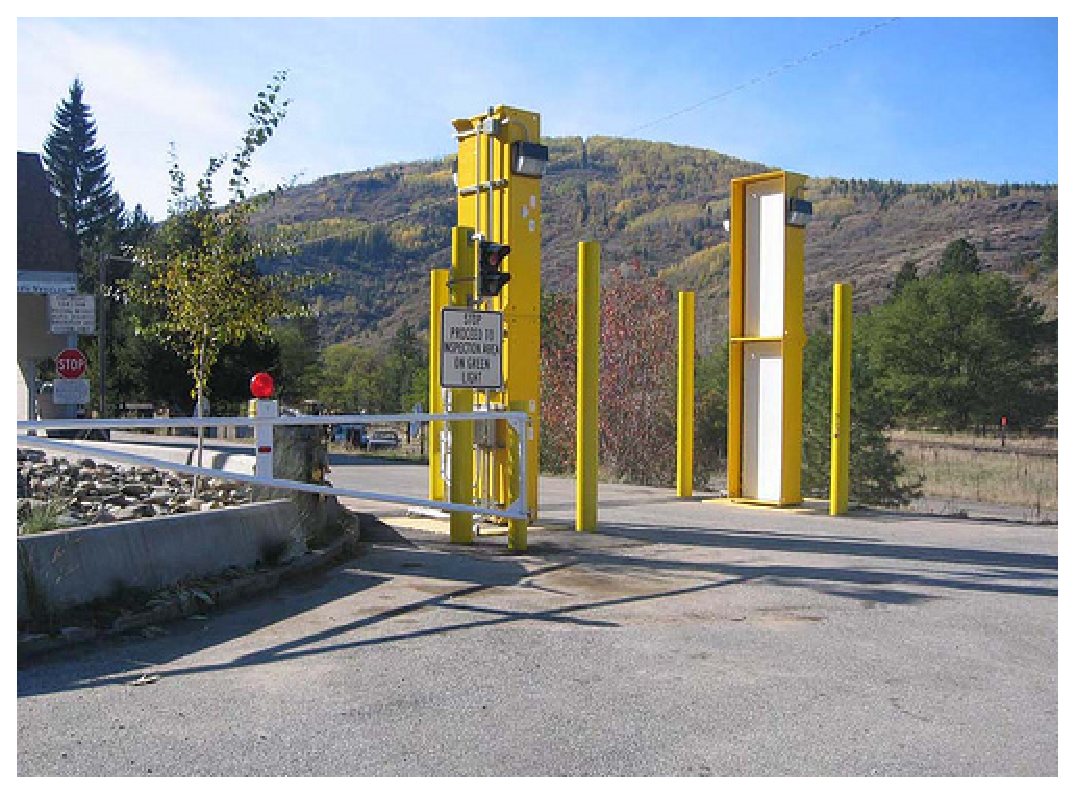
\includegraphics[width=\textwidth]{images/RPM8_Installed.eps}
			\label{fig:RPM8Installed}
			\caption{Installed RPM}
			\end{figure}
	\end{column}
\end{columns}
\end{frame}


%%%%%%%%%%%%%%%%%%%%%%%%%%%%%%%%%%%%%%%%%%%%%%%%%%%%%%%%%%%%%%%%%%%%%%%%%%%%%%%
\begin{frame}{Neutron Adsorption Interactions}
\begin{itemize}
	\item Desired reaction properties
	\begin{itemize}
		\item High probability of occurrence
		\item Ease of detecting reaction products
		\item Reaction products have a low pulse height deficit
	\end{itemize}
\end{itemize}
\begin{table}
	\tiny
	\begin{tabular}{ c | c c c} 
		Reaction                           & Q-Value (MeV) & Thermal Cross Section & Application \\
		\hline
		\hline
		${}^3He + n \to p +{}^3H$          & 0.756     & 5,330 & Proportional counter gas \\
		${}^6Li + n \to {}^3H + \alpha$    & 4.78      & 940 & Lithium glass scintillators \\
		${}^{10}B + n \to \alpha + {}^7Li$ & 2.31      & 3,840 & Plastic scintillators \\
		${}^{157}Gd + n \to \gamma$        &various    & 259,000 & various \\
	\end{tabular}
\end{table}
\end{frame}

%%%%%%%%%%%%%%%%%%%%%%%%%%%%%%%%%%%%%%%%%%%%%%%%%%%%%%%%%%%%%%%%%%%%%%%%%%%%%%%
\begin{frame}{Energy Deposition (Charged Particle)}
Products of ${}^6$Li neutron interaction are triton and alpha:
\begin{columns}[onlytextwidth]
\begin{column}{0.45\textwidth}
\begin{itemize}
	\small
	\item Alpha Energy: 2.05 MeV
	\item Triton Energy: 2.73 MeV
\end{itemize}
Alpha and tritons tend to deposit all of their energy in a small region
\end{column}
\begin{column}{0.45\textwidth}
	\begin{figure}
	\includegraphics[width=\textwidth]{images/PStarAStarRange.eps}
	\caption{Alpha and Triton Range (CSDA) \protect \cite{berger_estar_2005}}
	\label{fig:PStarAStarRange}
	\end{figure}
\end{column}
\end{columns}
\end{frame}

\subsection{Detector Requirements}
%%%%%%%%%%%%%%%%%%%%%%%%%%%%%%%%%%%%%%%%%%%%%%%%%%%%%%%%%%%%%%%%%%%%%%%%%%%%%%%
\begin{frame}{Detector Requirements}
DHS / DNDO (along with PNNL) has determined a set of objectives that replacement technologies should meet:
\begin{table}
	\tiny
	\begin{tabular}{c c }
	Parameter & Specification \\
	\hline
	\hline
	Absolute neutron detection efficiency & 2.5 cps/ng of ${}^{252}Cf$ (in specified test configuration) \\
	Intrinsic gamma-neutron detection efficiency & $ \epsilon_{int,\gamma}\leq 10^{-6}$ \\
	Gamma absolute rejection ratio for neutrons (GARRn) & $ 0.9 \leq \text{ GARRn }\leq$ 1.1 at 10 mR/h exposure \\
	Cost &  \$ 30,000 per system \\
	\hline
	\end{tabular}
\end{table}
\end{frame}

%%%%%%%%%%%%%%%%%%%%%%%%%%%%%%%%%%%%%%%%%%%%%%%%%%%%%%%%%%%%%%%%%%%%%%%%%%%%%%%
\begin{frame}{Absolute Neutron Efficiency}
\newtheorem{thm1}{Absolute Neutron Efficiency}
\begin{thm1}<1->
$$\epsilon_{abs} = \frac{\text{Counts}}{\text{Quanta Radiation Emitted}}\; \; \protect \cite{knoll_radiation_2009} $$
Constraint:
$$\epsilon_{abs} \geq 2.5\; \text{cps per ng}\; {}^{252}\text{Cf}$$
\end{thm1}
Test configuration is defined to be 1 ng ${}^{252}$Cf surrounded by 0.5 cm of lead and 2.5 cm of HDPE, with the detector midpoint 2 m from the source \cite{kouzes_alternative_2010}
\end{frame}


%%%%%%%%%%%%%%%%%%%%%%%%%%%%%%%%%%%%%%%%%%%%%%%%%%%%%%%%%%%%%%%%%%%%%%%%%%%%%%%
\begin{frame}{Intrinsic Gamma-Neutron Detection Efficiency}
\newtheorem{thm2}{Intrinsic Gamma-Neutron Detection Efficiency}
\begin{thm2}<1->
$$\epsilon_{int,n \gamma} = \frac{\text{Counts}}{\text{Quanta Radiation Crossing Detector}} \; \protect \cite{kouzes_alternative_2010} $$
Constraint:
$$ \epsilon_{int,n \gamma} \leq 10^{-6} $$
\end{thm2}
\begin{itemize}
	\item Counts over quanta crossing the detector
	\item Measured from a source that produces a 10 mR/hr field
\end{itemize}
\end{frame}

%%%%%%%%%%%%%%%%%%%%%%%%%%%%%%%%%%%%%%%%%%%%%%%%%%%%%%%%%%%%%%%%%%%%%%%%%%%%%%%
\begin{frame}{Gamma Absolute Rejection Ratio}
\newtheorem{thm3}{GARRn}
\begin{thm3}<1->
$$ GARRn = \frac{\epsilon_{\gamma,abs}}{\epsilon_{n,abs}} \; \protect \cite{kouzes_alternative_2010} $$
Constraint:
$$ 0.9 \leq GARRn \leq 1.1 $$
\end{thm3}
The detector's performance should change by no more than 10\% in a strong gamma field
\begin{itemize}
	\item GARRn is measured by exposing the detector to a 10 mR/hr gamma field while exposed to neutron source
	\item Count rate is measured when the gamma source is no longer present
	\item Difference determines the GARRn
\end{itemize}
\end{frame}

%%%%%%%%%%%%%%%%%%%%%%%%%%%%%%%%%%%%%%%%%%%%%%%%%%%%%%%%%%%%%%%%%%%%%%%%%%%%%%%
%                                                                             %
%                                PREVIOUS WORK                                %
%                                                                             %
%%%%%%%%%%%%%%%%%%%%%%%%%%%%%%%%%%%%%%%%%%%%%%%%%%%%%%%%%%%%%%%%%%%%%%%%%%%%%%%
\subsection{Previous Work}

%%%%%%%%%%%%%%%%%%%%%%%%%%%%%%%%%%%%%%%%%%%%%%%%%%%%%%%%%%%%%%%%%%%%%%%%%%%%%%%
\begin{frame}{Replacement Technologies (Boron)}
\begin{columns}[onlytextwidth]
\begin{column}{0.45\textwidth}
\begin{itemize}
	\small
	\item Boron Straw Tubes (Proportional Technology) \cite{kouzes_boron-lined_2012}
	\begin{itemize}
		\tiny
		\item Count rate meets requirements
		\item Gamma rejection is estimated to be $4x10^{-9}$
		\item GARRn within desired range
	\end{itemize}
	\small
	\item Boron Triflouride Gas Detectors (LND) \cite{kouzes_bf3_2009}
	\begin{itemize}
		\tiny
        \item Two tubes are marginally able to replace one ${}^3$He tube
		\item BF${}_3$ Tubes require 2200V to operate than ${}^3$He tubes (1000 V)
		\item BF${}_3$ Tubes require less pressure than ${}^3$He tubes
	\end{itemize}
\end{itemize}
\end{column}
\begin{column}{0.45\textwidth}
	\begin{figure}
	\centering
		\includegraphics[height=0.25\textheight]{images/B10StrawFibers.eps}
		\caption{ ${}^{10}$B Straw Fibers}
		\label{fig:B10StrawFibers}
		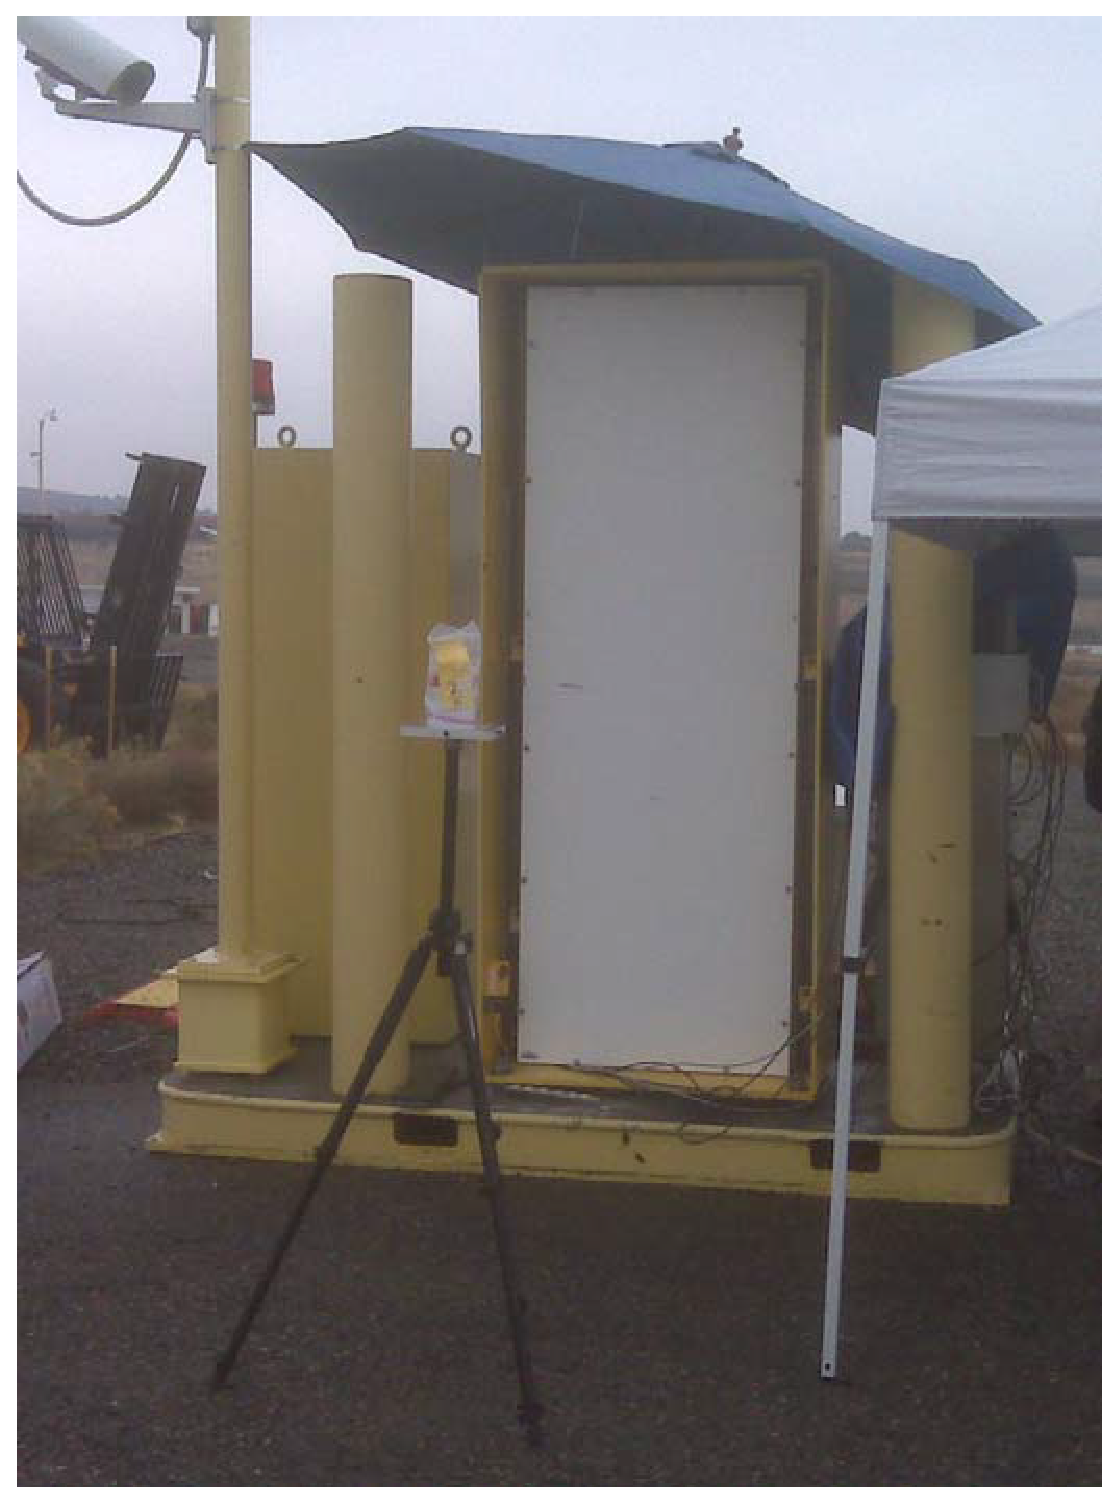
\includegraphics[height=0.25\textheight]{images/BF3Test.eps}
		\caption{PNNL test of BF${}_3$ Detector}
		\label{fig:BF3PNNLTest}
	\end{figure}
\end{column}
\end{columns}
\end{frame}

%%%%%%%%%%%%%%%%%%%%%%%%%%%%%%%%%%%%%%%%%%%%%%%%%%%%%%%%%%%%%%%%%%%%%%%%%%%%%%%
\begin{frame}{Replacement Technologies (Lithium)}
\begin{columns}[onlytextwidth]
\begin{column}{0.45\textwidth}
\begin{itemize}
	\small
	\item LiF:ZnS coated Paddles (IAT) \cite{kouzes_lithium_2010}
	\begin{itemize}
		\item Did not fulfill the neutron count rate
		\item Adequate gamma ray rejection
		\item Passed the GARRn
	\end{itemize}
	\small
	\item NucSafe Glass Fibers\cite{kouzes_alternative_2010}
	\begin{itemize}
		\item Tested with a scale model, 1.72 cps
		\item Three filter levels for GARRn
		\begin{itemize}
			\tiny
			\item Conservative filter passed GARRn, failed count rate
			\item Other filters failed GARRn
		\end{itemize}
	\end{itemize}
\end{itemize}
\end{column}
\begin{column}{0.45\textwidth}
	\begin{figure}
		\includegraphics[height=0.25\textheight]{images/LiFZnSPaddle.eps}
		\caption{${}^6$LiF:ZnS Paddle}
		\label{fig:LifZnSPaddle}
		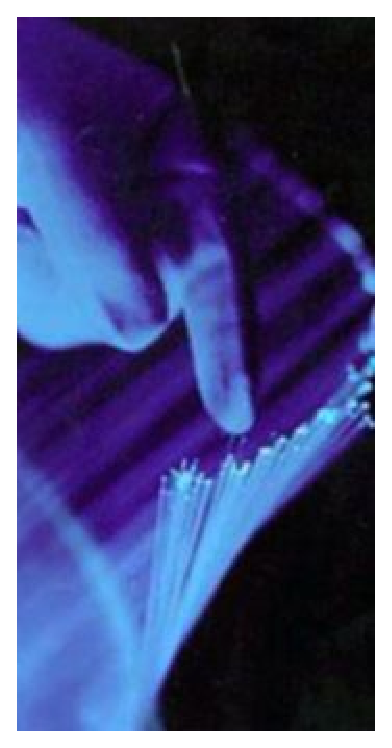
\includegraphics[height=0.25\textheight]{images/NucSafeFibers.eps}
		\caption{NucSafe Fibers}
		\label{fig:NucSafeFibers}
	\end{figure}
\end{column}
\end{columns}
\end{frame}

%%%%%%%%%%%%%%%%%%%%%%%%%%%%%%%%%%%%%%%%%%%%%

\section{Previous Work}
\label{sec:PreviousWork}
Previous work on the energy deposition of thin focused on spectra measurements from fabricated films as wells as single collision energy loss spectra.
A sequence of 10\% \iso{Li}{6}F, 5\% PPOPOPOP films in a PS matrix cast to thickness between 15 and 600 $\mu$m where fabricated and the response was measured from a gamma source as well as a neutron source.
These experiment results are shown in \ref{sec:SpectraMeasurements}.

\subsection{Spectra Measurements}
\label{sec:SpectraMeasurements}
Evidence that the secondary electrons contribute to energy loss can be seen in Figure \ref{fig:SpectraFeatures} where there is an increase in the endpoint of the spectra as films become thicker.
This increase in the spectra endpoint is indicative of the film producing more light, and as the light collection geometry remained constant the increase in the endpoint is attributed to a larger energy deposition in the 50 $\mu$m film compared to the 15 $\mu$m or 25 $\mu$m film.
%%%%%%%%%%%%%%%%%%%% Figures %%%%%%%%%%%%%%%%%%%%%%%%
\begin{figure}[h]
    \centering
    \begin{subfigure}[b]{0.45\figurewidth}
        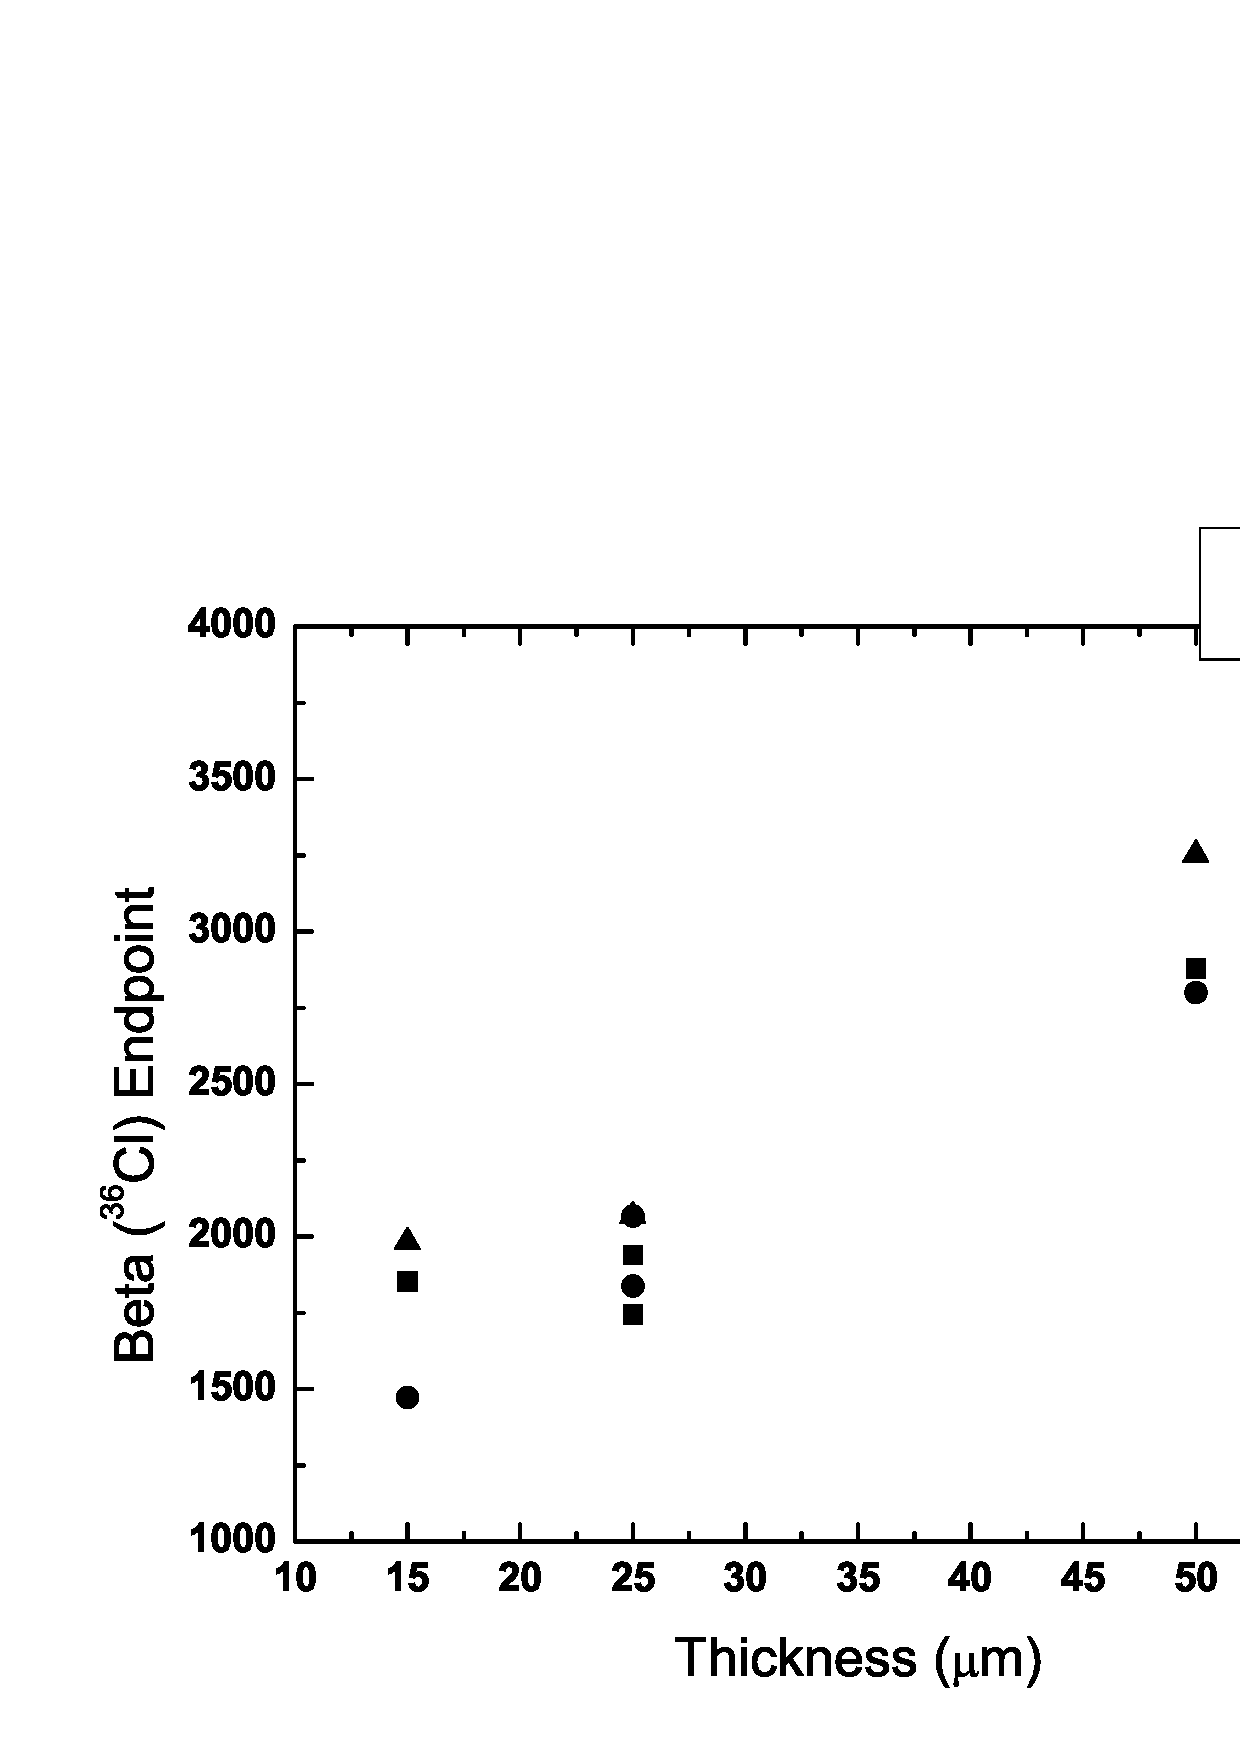
\includegraphics[width=\textwidth]{Beta}
        \caption{Beta Spectra Endpoints for a 5\% PS film}
    \end{subfigure}
    \begin{subfigure}[b]{0.45\figurewidth}
        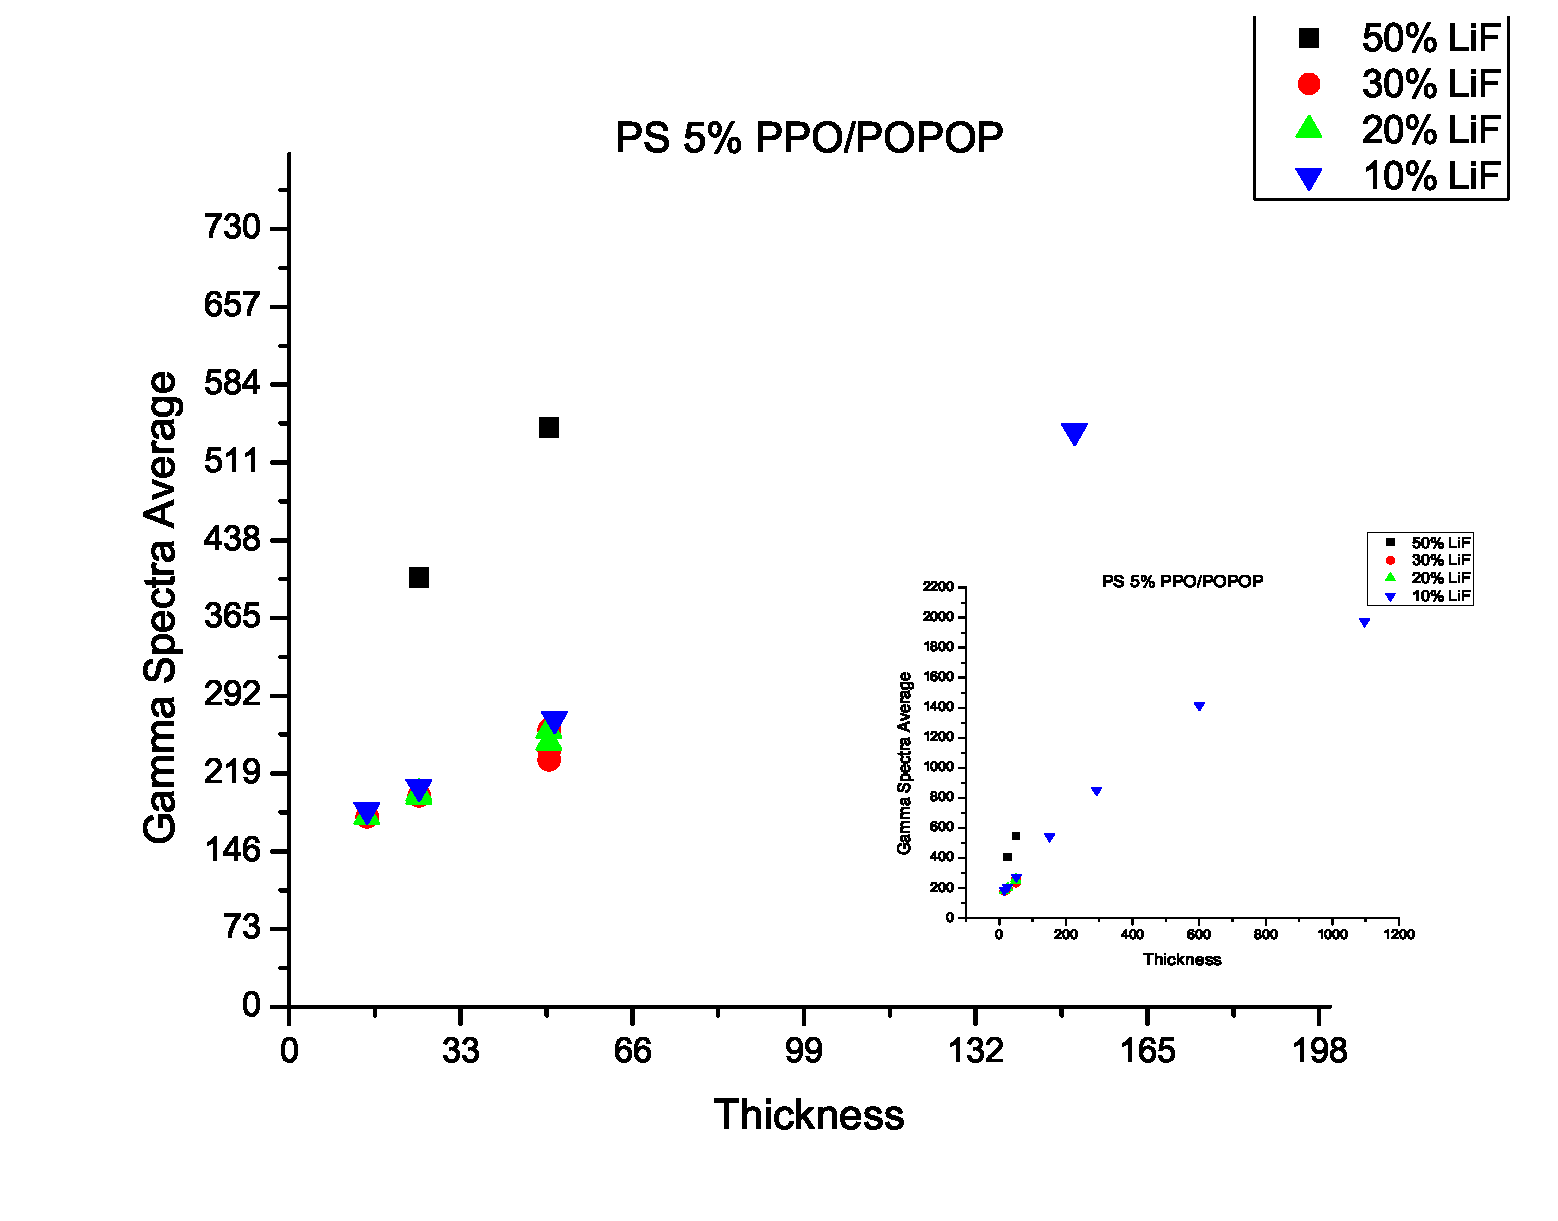
\includegraphics[width=\textwidth]{PS-5PPOPOPOP_GammaAvg}
        \caption{Gamma Spectra Averages for PS films}
    \end{subfigure}
    \caption{Spectra properties as a function of film thickness}
    \label{fig:SpectraFeatures}
\end{figure}
Figure \ref{fig:GammaIntrNeutronCounts} shows the intrinsic efficiency of these film (from spectra obtained from a \iso{Co}{60} source).
As the film thickness increases the pulse height discriminator at which an intrinsic efficiency of one in a million ($\epsilon_{int,\gamma} \le 10^{-6}$) is reached also increase.
The neutron spectra (shown in the solid lines) does not increase in light yield with increasing thickness, further providing an indication that the thickness of the films can be optimized to maximize the neutron count rates\footnote{The neutron count rate is increased with thickness by the increased mass of the detector} while minimizing the response of the detector to photons.
%%%%%%%%%%%%%%%%%%%% Figures %%%%%%%%%%%%%%%%%%%%%%%%
\begin{figure}[ht]
    \centering
    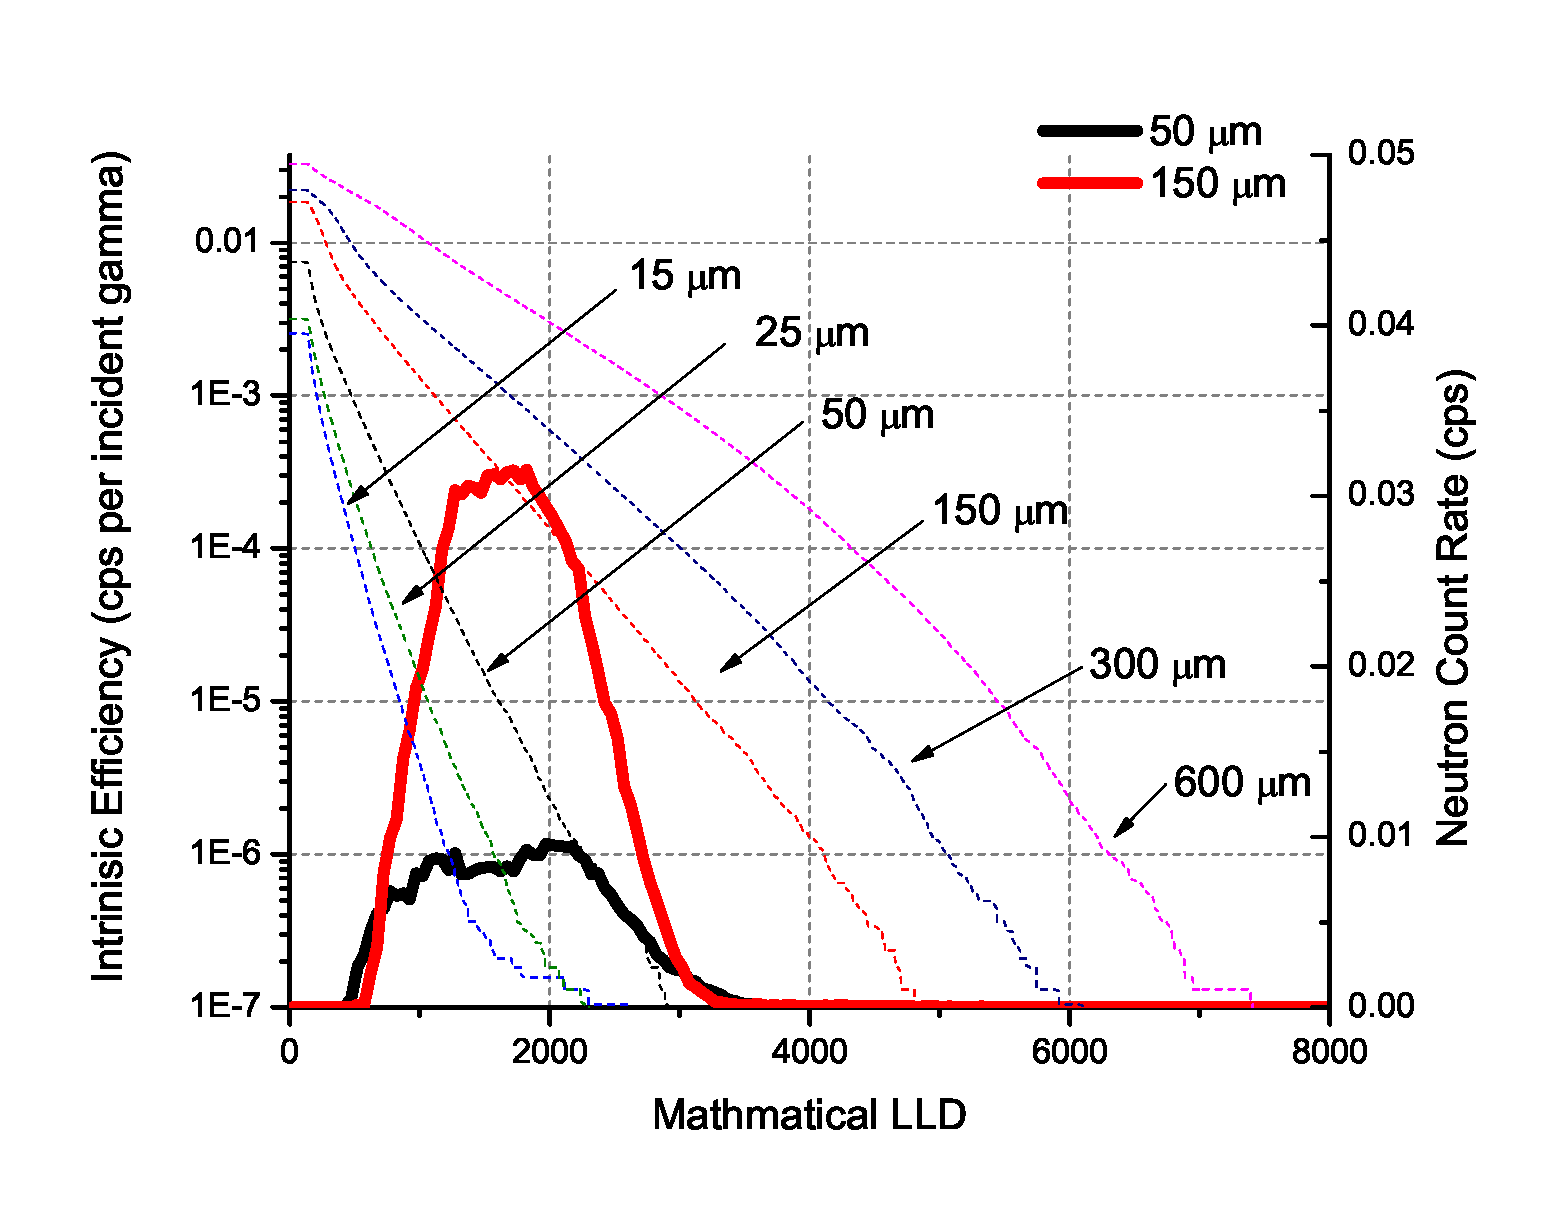
\includegraphics[width=\textwidth]{PS_IntEff_LiF20_PPO5}
    \caption{Gamma intrinsic efficiency (dashed lines) plotted against neutron counts (solid)}
    \label{fig:GammaIntrNeutronCounts}
\end{figure}

\subsection{Single Collision Energy Loss}

Single collision energy loss spectra provide the probability that that a given collision will result in an energy loss of Q.
Provided a spectra of secondary electrons from either the Compton scattered electron or the \iso{Li}{6} reaction products it is then possible to determine the average energy loss per collision.
A single collision energy loss spectra for water is shown in Figure \ref{fig:TurnerELoss}.
For low electron energies ($<$ 50 eV) it is very probable that the electron will lose a majority of its energy in a single collision.
For higher electron energies, however, the electrons tend to lose a lower fraction of there total energy. 
A Compton scattered photon, with an energy in the MeV range, will then lose far less energy per collision than an electron (in the low keV range) liberated from the passage of a neutron reaction product through the material.
%%%%%%%%%%%%%%%%%%%% Figures %%%%%%%%%%%%%%%%%%%%%%%%
\begin{figure}[ht]
    \centering
    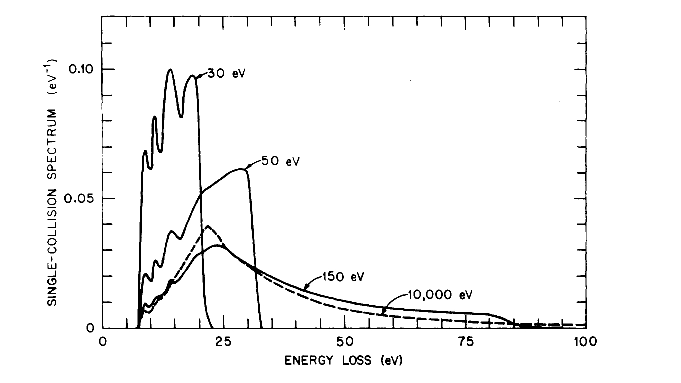
\includegraphics[width=\textwidth]{Turner_Fig2_SingleCollisionELoss}
    \caption{Single-collision energy loss spectra for electrons in water \protect\cite{turner_comparative_1982}}
    \label{fig:TurnerELoss}
\end{figure}
When the average and median energy transfer are plotted as a function of incident electron energy (Figure \ref{fig:TurnerETransfer}) the difference in the energy loss spectra becomes more apparent.
For low energies (up to an incident electron energy of 100 eV) the average and median energy transfer are roughly equal to each other, about half of the incident electron.
Past 100 eV average energy increases faster than the median energy transfer implying that while a few collisions result in large energy transfers most of the collisions do not.
It is also interesting to note that the average and median do not increase linearly with the incident energy past 100 eV (the ordinate axis is a log scale). 
In fact, the average energy transferred per collision is mostly bounded by 60 eV even for incident electron energies of \~10 keV.
This is significant because it implies that high energy electrons from photon events will deposit a small fraction of their energy in the material.
%%%%%%%%%%%%%%%%%%%% Figures %%%%%%%%%%%%%%%%%%%%%%%%
\begin{figure}[ht]
    \centering
    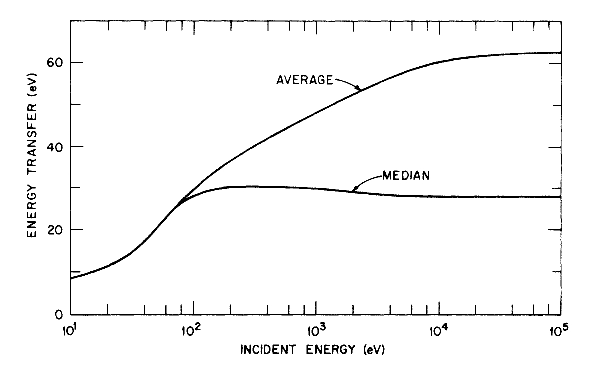
\includegraphics[width=\textwidth]{Turner_Fig3_AvgMedianETransfer}
    \caption{Average and median energy transfer in liquid water as functions of incident-electron energy \protect\cite{turner_comparative_1982}}
    \label{fig:TurnerETransfer}
\end{figure}

%%%%%%%%%%%%%%%%%%%%%%%%%%%%%%%%%%%%%
\subsection{Introduction to GEANT4}

GEANT4 (GEomentry ANd Tracking) is a free, open source Monte Carlo based physics simulation toolkit developed and mainted at CERN widely used in the physics community.
A GEANT4 simulation starts with a run which contains a set number of events.
An event is particular process of intrest to the user, such as shooting a single particle at a detector. 
Typical usage might be to have a run be firing 1,000 neutrons at a detector, were each neutron is a single event.


\subsubsection{Organization of the GEANT4 Toolkit}
The GEANT4 toolkit is divided into eight (8) class categories:
\begin{itemize}
    \item Run and Event - generation of events and secondary particles.
    \item Tracking and Track - transport of a particle by analyzing the factors limiting the step size and by applying the revelant physics models.
    \item Geometry and Magnetic Field - the geometical defination of a detector (including the computation of the distnances to solids) as wells as the management of magnetic fields.
    \item Particle Defination and Matter - defination of particles and matter.
    \item Hits and Digitization - the creation of hits and their use for digitization in order to model a detectors readout response.
    \item Visualization - the visualziation of a simulation inlcuding the solid geometry, trajectories and hits.
    \item Interaface - the intearctions between the toolkit and graphical user interafaces and well as external software.
\end{itemize}

There are then three classes which must be implemented by the user in order use the toolkit. These classes are:
\begin{itemize}
    \item \verb+G4VuserDetectorConstruction+ which defines the geometry of the simulation,
    \item \verb+G4VUserPhysicsList+ which defines the physics of the simulation, and
    \item \verb+G4VUserPriamryGeneratorAction+ which defines the generation of primary events.
\end{itemize}
Five additional classes are avaible for further control over the simulation:
\begin{itemize}
    \item \verb+G4UserRunAction+ which allows for user actions
\end{itemize}

% !TEX TS-program = pdflatex
% !TEX encoding = UTF-8 Unicode

% Matthew Urffer Master Thesis
% 
% Methods
%
\section{Spectra Methods}

%%%%%%%%%%%%%%%%%%%%%%%%%%%%%%%%%%%%%%%%%%%%%%%%%%%%%%%%%%%%%%%%%%%%%%%%%%%%%%%
%                                                                             %
%                                   FACILITIES                                %
%                                                                             %
%%%%%%%%%%%%%%%%%%%%%%%%%%%%%%%%%%%%%%%%%%%%%%%%%%%%%%%%%%%%%%%%%%%%%%%%%%%%%%%

\subsection{Facilities}
%%%%%%%%%%%%%%%%%%%%%%%%%%%%%%%%%%%%%%%%%%%%%%%%%%%%%%%%%%%%%%%%%%%%%%%%%%%%%%%
\begin{frame}{Button Sources}
	\centering
	Alpha Sources
	\begin{table}[h]
		\tiny
		\begin{tabular}{c | c c}
		Source & Half-Life & Energy (MeV) \\
		\hline
		\hline
		${}^{232}$Th & $1.4\times10^{10}$ yr & 4.012 \\
		${}^{240}$Pu & $6.5\times10^{3}$ yr & 5.17 (76\%) 5.12 (24\%) \\
		${}^{241}$Am & 433 yr & 5.48 (85\%) 5.44 (12\%) \\
		${}^{239}$Pu, ${}^{241}$Am, ${}^{244}$Cm  & various & various \\
		\hline
		\end{tabular}
	\end{table}
	Beta Sources
	\begin{table}[h]
		\tiny
		\begin{tabular}{c | c c}
		Source & Half-Life & Endpoint Energy (MeV)\\
		\hline
		\hline
		${}^{14}$C &  5,730 yr & 0.156 \\
		${}^{36}$Cl & $3.08\times10^{5}$ yr & 0.714 \\
		${}^{36}$Ni &  92 yr & 0.067 \\
		${}^{99}$Tc & $2.12\times10^{5}$ yr & 0.292 \\
		\hline
		\end{tabular}
	\end{table}
\end{frame}

%%%%%%%%%%%%%%%%%%%%%%%%%%%%%%%%%%%%%%%%%%%%%%%%%%%%%%%%%%%%%%%%%%%%%%%%%%%%%%%
\begin{frame}{Gamma Irridiator}
\begin{columns}[onlytextwidth]
\begin{column}{0.45\textwidth}
	\begin{itemize}
		\item Desire a 10 mR/hr Gamma Field
		\item Solution is 1 100 $\mu$Ci ${}^{60}$Co source
		\item Shielded by lead
	\end{itemize}
\end{column}
\begin{column}{0.45\textwidth}
	\centering
	\begin{figure}
		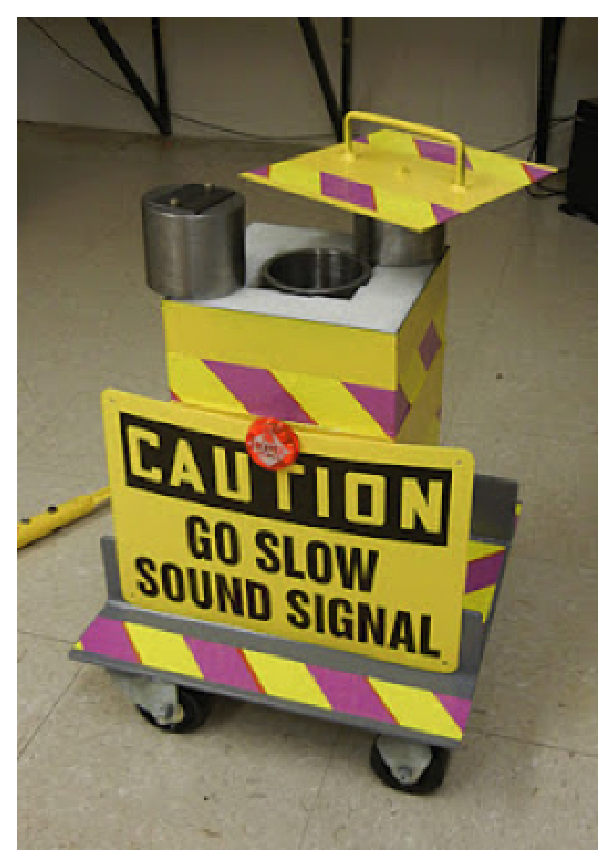
\includegraphics[width=0.8\textwidth]{images/GammaIrridiator.eps}
		\label{fig:GammaIrridiator}
		\caption{Gamma Irridiator}
	\end{figure}
\end{column}
\end{columns}
\end{frame}

%%%%%%%%%%%%%%%%%%%%%%%%%%%%%%%%%%%%%%%%%%%%%%%%%%%%%%%%%%%%%%%%%%%%%%%%%%%%%%%
\begin{frame}{Neutron Irridiator}
\begin{columns}[onlytextwidth]
\begin{column}{0.45\textwidth}
	\small
	\begin{itemize}
		\item Source is 0.59 $\mu$g ${}^{252}$Cf
		\item Encased in HDPE Box
		\item Two detector wells
		\begin{itemize}
			\tiny
			\item Lead Well
			\item Cadmium Well
		\end{itemize}
	\end{itemize}
\end{column}
\begin{column}{0.45\textwidth}
	\begin{figure}
		\centering
		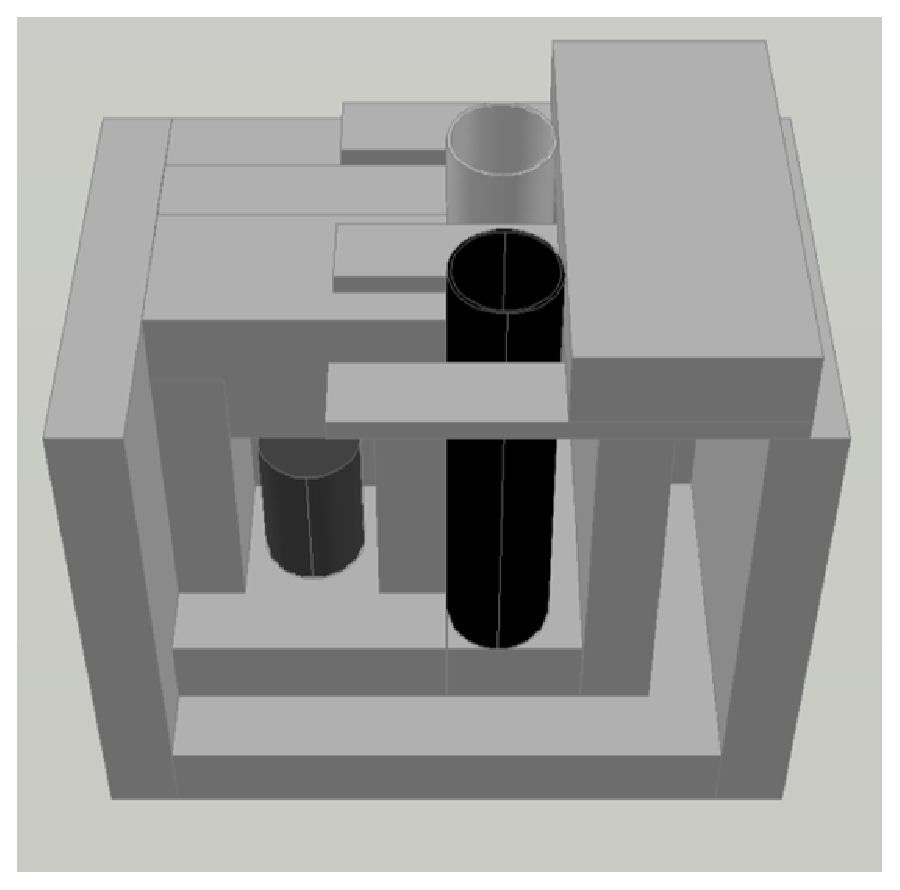
\includegraphics[height=0.25\textheight]{images/NeutronIrridiator_CAD.eps}
		\caption{CAD Rendering of Neutron Irridiator}
		\label{fig:NeutronIrridiatorCAD}
		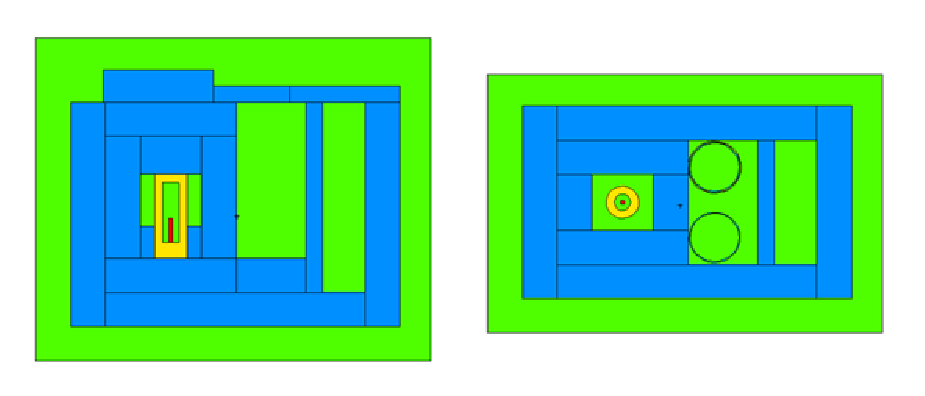
\includegraphics[height=0.25\textheight]{images/NeutronIrridiator_MCNP.eps}
		\caption{MCNPX Rendering of Neutron Irridiator}
		\label{fig:NeutronIrridiatorMNCPX}
	\end{figure}
\end{column}
\end{columns}
\end{frame}

%%%%%%%%%%%%%%%%%%%%%%%%%%%%%%%%%%%%%%%%%%%%%%%%%%%%%%%%%%%%%%%%%%%%%%%%%%%%%%%
\begin{frame}{Neutron Irridiator (Spectra)}
\begin{columns}[onlytextwidth]
\begin{column}{0.45\textwidth}
	\begin{itemize}
		\small
		\item Lead Well
		\begin{itemize}
			\tiny
			\item Neutrons of all energies
			\item Lead to match photon attenuation of cadmium
		\end{itemize}
		\small
		\item Cadmium Well
		\begin{itemize}
			\tiny
			\item Cadmium cutoff is about 0.5 eV
			\item Well response is to fast neutrons
			\item Shielding of photons from cadmium
		\end{itemize}
		\small 
		\item Subtraction is preformed between the two response to extract the response from thermal neutrons
	\end{itemize}
\end{column}
\begin{column}{0.45\textwidth}
	\begin{figure}
		\centering
		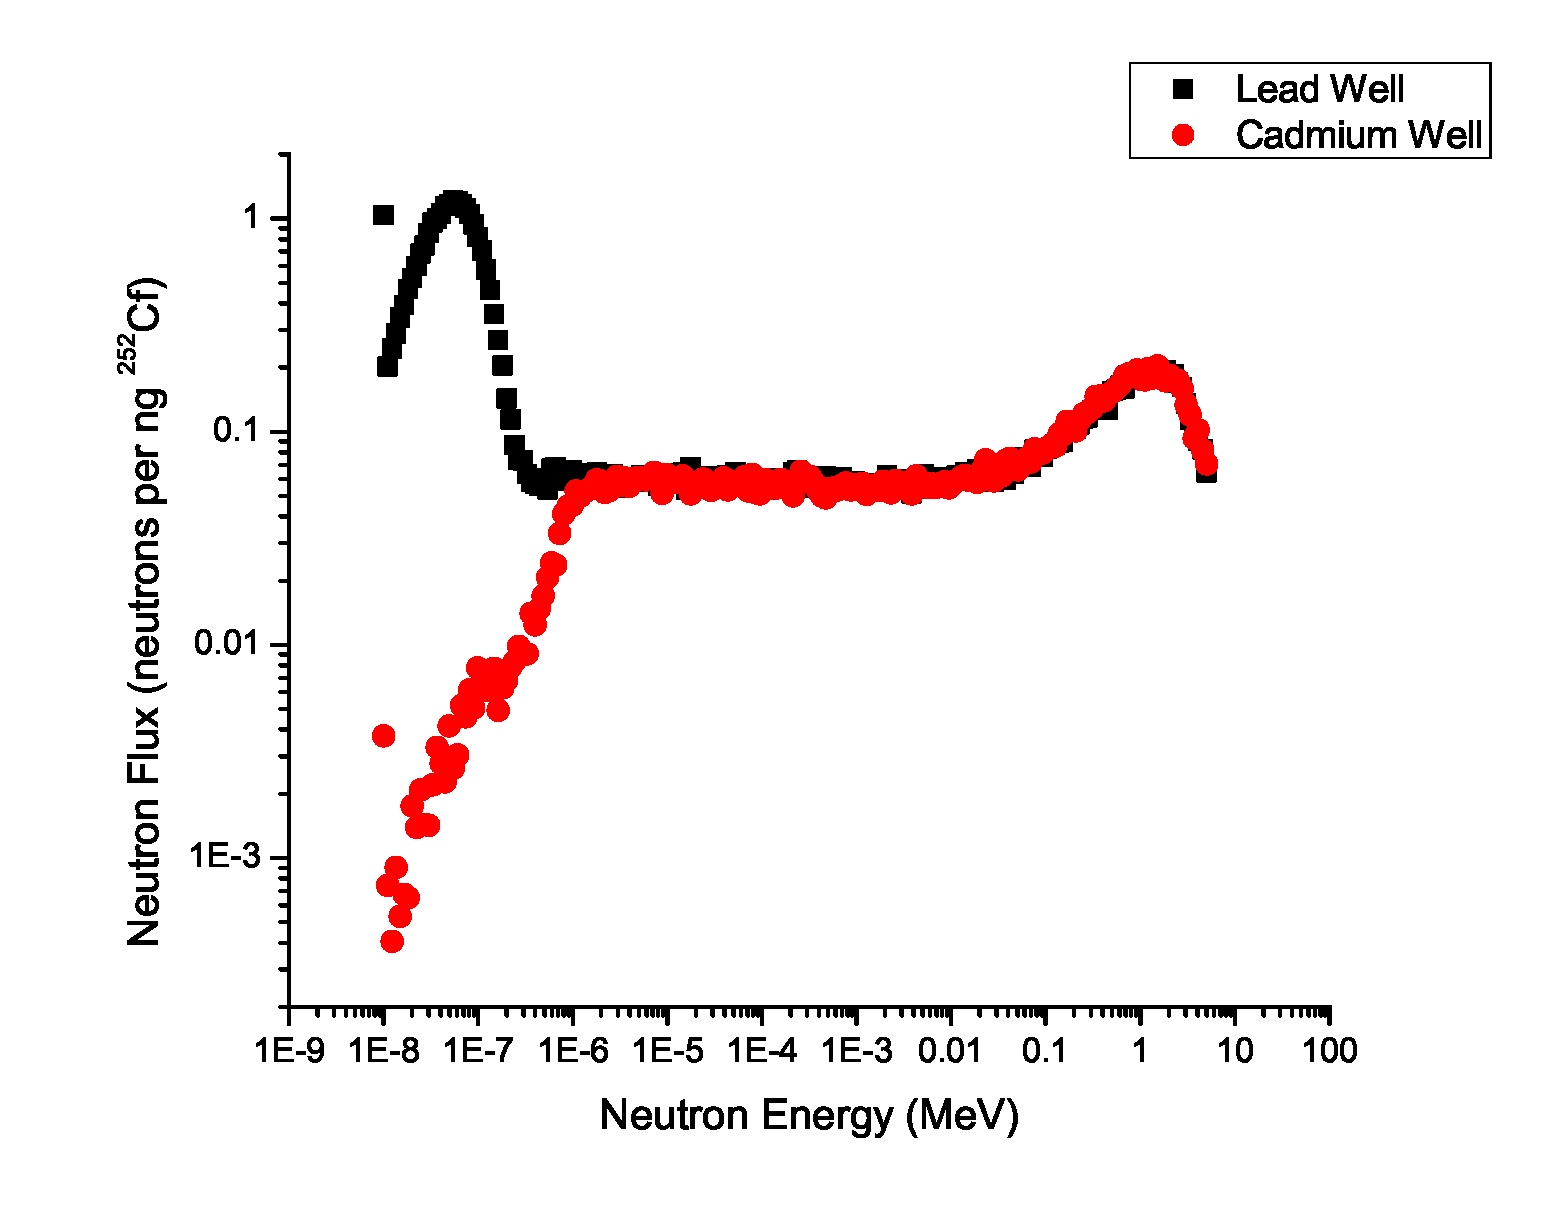
\includegraphics[height=\textwidth]{images/Graph19N.eps}
		\caption{Simulated Lead and Cadmium Well Spectra}
		\label{fig:SimPbCdSpectra}
	\end{figure}
\end{column}
\end{columns}
\end{frame}
%%%%%%%%%%%%%%%%%%%%%%%%%%%%%%%%%%%%%%%%%%%%%%%%%%%%%%%%%%%%%%%%%%%%%%%%%%%%%%%
\begin{frame}{Spectra Electronics}
\begin{columns}[onlytextwidth]
\begin{column}{0.45\textwidth}
	\small 
	Measurement Protocol
	\begin{itemize}
		\tiny
		\item Verify instrument gains are stable
		\begin{itemize}
			\tiny
			\item GS20 (${}^6$Li glass) is used as the standard
			\item Set voltage and coarse gain, adjust fine gain
		\end{itemize}
		\tiny
		\item Obtain a spectra from an alpha (${}^{241}$Am) 
		\item Obtain a spectra from a beta (${}^{36}$Cl)
		\item Obtain a lead well neutron spectra
		\item Obtain a cadmium well neutron spectra
		\item Obtain a gamma irridiator spectra
	\end{itemize}
\end{column}
\begin{column}{0.45\textwidth}
	\begin{figure}
		\centering
		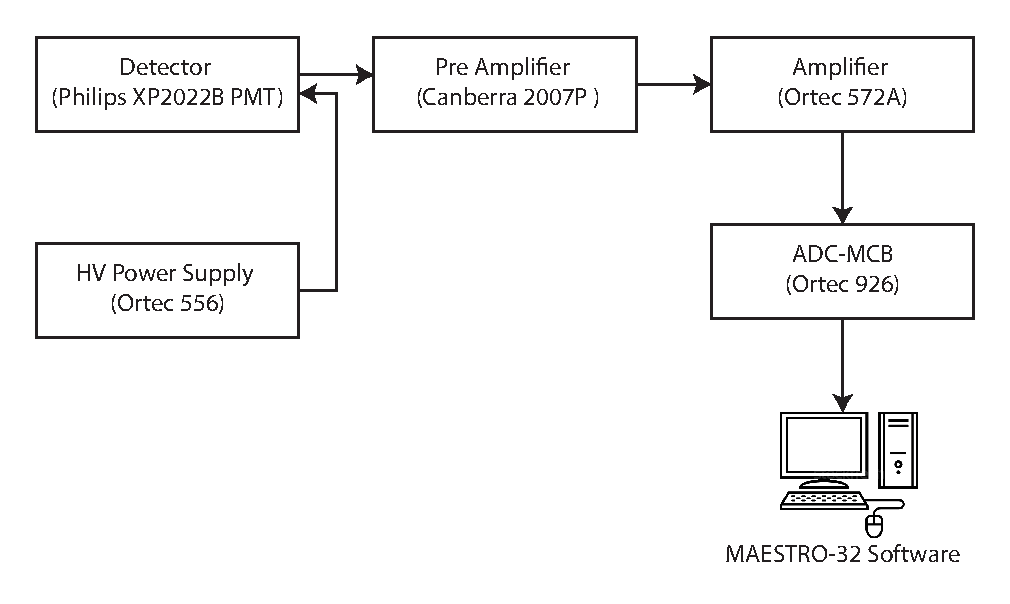
\includegraphics[height=0.5\textwidth]{images/ElectronicsSpectra.eps}
		\caption{Electronic Setup for Spectra}
		\label{fig:ElectronicsSpectra}
	\end{figure}
\end{column}
\end{columns}
\end{frame}
%%%%%%%%%%%%%%%%%%%%%%%%%%%%%%%%%%%%%%%%%%%%%%%%%%%%%%%%%%%%%%%%%%%%%%%%%%%%%%%
%                                                                             %
%                             ANALYSIS METHDOS                                %
%                                                                             %
%%%%%%%%%%%%%%%%%%%%%%%%%%%%%%%%%%%%%%%%%%%%%%%%%%%%%%%%%%%%%%%%%%%%%%%%%%%%%%%
\subsection{Analysis Methods}
%%%%%%%%%%%%%%%%%%%%%%%%%%%%%%%%%%%%%%%%%%%%%%%%%%%%%%%%%%%%%%%%%%%%%%%%%%%%%%%
\begin{frame}{Spectra Average}
	\begin{itemize}
		\item Thin films do not have clearly define features
		\item Spectra averages defined to create a feature
	\end{itemize}
	\newtheorem{thm4}{Spectra Average}
	\begin{thm4}<1->
		$$<\mu> = \frac{\int_{0}^{\infty}x f(x)dx}{\int_{0}^{\infty}f(x)dx} $$
		where:
		\begin{itemize}
			\tiny
			\item $<\mu>$ is the average of the spectra
			\item $f(x)$ is the spectra
			\item $x$ is a channel number
		\end{itemize}
	\end{thm4}
\end{frame}
%%%%%%%%%%%%%%%%%%%%%%%%%%%%%%%%%%%%%%%%%%%%%%%%%%%%%%%%%%%%%%%%%%%%%%%%%%%%%%%
\begin{frame}{Pulse Height Deficit}
	\newtheorem{thm5}{Pulse Height Deficit}
	\begin{thm5}<1->
	\tiny
	$$ PHD_{GS20} = \frac{\dfrac{n_{peak}}{4.78\;\text{MeV}}}{\dfrac{CE_\gamma}{1.038\;\text{MeV}}} $$
		where:
		\begin{itemize}
			\tiny
			\item $PHD_{GS20}$ is the pulse height deficit for GS20
			\item $n_{peak}$ is the location of the peak in the neutron spectra
			\item $CE_\gamma$ is the Compton Edge of the Gamma Spectra
		\end{itemize}
	\end{thm5}
	\newtheorem{thm6}{Pulse Height Deficit (Sample)}
	\begin{thm6}<1->
	\tiny
	$$ PHD_{Sample} = PHD_{GS20} \frac{<n>_{sample}}{<n>_{GS20}} $$
		where:
		\begin{itemize}
			\tiny
			\item $PHD_{GS20}$ is the pulse height deficit for GS20
			\item $<n>_{sample}$ is the average of the sample's neutron spectra
			\item $<n>_{GS20}$ is the average of GS20's neutron spectra
		\end{itemize}
	\end{thm6}
\end{frame}
%%%%%%%%%%%%%%%%%%%%%%%%%%%%%%%%%%%%%%%%%%%%%%%%%%%%%%%%%%%%%%%%%%%%%%%%%%%%%%%
\begin{frame}{Light Yield}
	\newtheorem{thm7}{Light Yield}
	\begin{thm7}<1->
	\tiny
	$$ LY_{n} = 3,800 \frac{\text{Photons}}{\text{MeV}}\frac{<n>_{sample}}{<n>_{GS20}} $$
	$$ LY_{\beta} = 3,800 \frac{\text{Photons}}{\text{MeV}}\frac{<\beta>_{sample}}{<\beta>_{GS20}} $$
	$$ LY_{\gamma} = 3,800 \frac{\text{Photons}}{\text{MeV}}\frac{<\gamma>_{sample}}{<\gamma>_{GS20}} $$
		where:
		\begin{itemize}
			\tiny
			\item $<n>_{sample}$ is the average of the sample's neutron spectra
			\item $<n>_{GS20}$ is the average of GS20's neutron spectra
			\item $<\beta>_{sample}$ is the average of the sample's beta (${}^{36}$Cl) spectra
			\item $<\beta>_{GS20}$ is the average of GS20's bet (${}^{36}$Cl) spectra
			\item $<\gamma>_{sample}$ is the average of the sample's gamma (${}^{60}$Co) spectra
			\item $<\gamma>_{GS20}$ is the average of GS20's gamma (${}^{60}$Co) spectra
		\end{itemize}
	\end{thm7}
\end{frame}
%%%%%%%%%%%%%%%%%%%%%%%%%%%%%%%%%%%%%%%%%%%%%%%%%%%%%%%%%%%%%%%%%%%%%%%%%%%%%%%
\begin{frame}
	\newtheorem{thm8}{Gamma Intrinsic Efficiency}
	\begin{thm8}<1->
		$$ \epsilon_{int,\gamma} = \frac{\int_{MLLD}^{\infty}{f(x)dx}}{\text{Particles Incident}} $$
	where:
	\begin{itemize}
		\tiny
		\item $MLLD$ is the mathematical lower level discriminator
		\item $f(x)$ is the spectra
		\item $\text{Particles Incident}$ is the number of incident particles
	\end{itemize}
	\end{thm8}
	\newtheorem{rmk1}{Mathematical Lower Level Discriminator}
	\begin{rmk1}
		\tiny
		Mathematical lower level discriminator (MLLD) is defined to be the channel at which $\epsilon_{int,\gamma} \leq 10^{-6}$
	\end{rmk1}

	\begin{itemize}
		\tiny
		\item MLLD for a film is determined from a ${}^{60}$Co measurement
		\item Source produces a 10 mR/hr field at detector surface
		\item Particles incident determined from simulation
	\end{itemize}
\end{frame}
%%%%%%%%%%%%%%%%%%%%%%%%%%%%%%%%%%%%%%%%%%%%%%%%%%%%%%%%%%%%%%%%%%%%%%%%%%%%%%%
\begin{frame}{Gamma Intrinsic Efficiency Example I}
	\begin{figure}
		\centering
		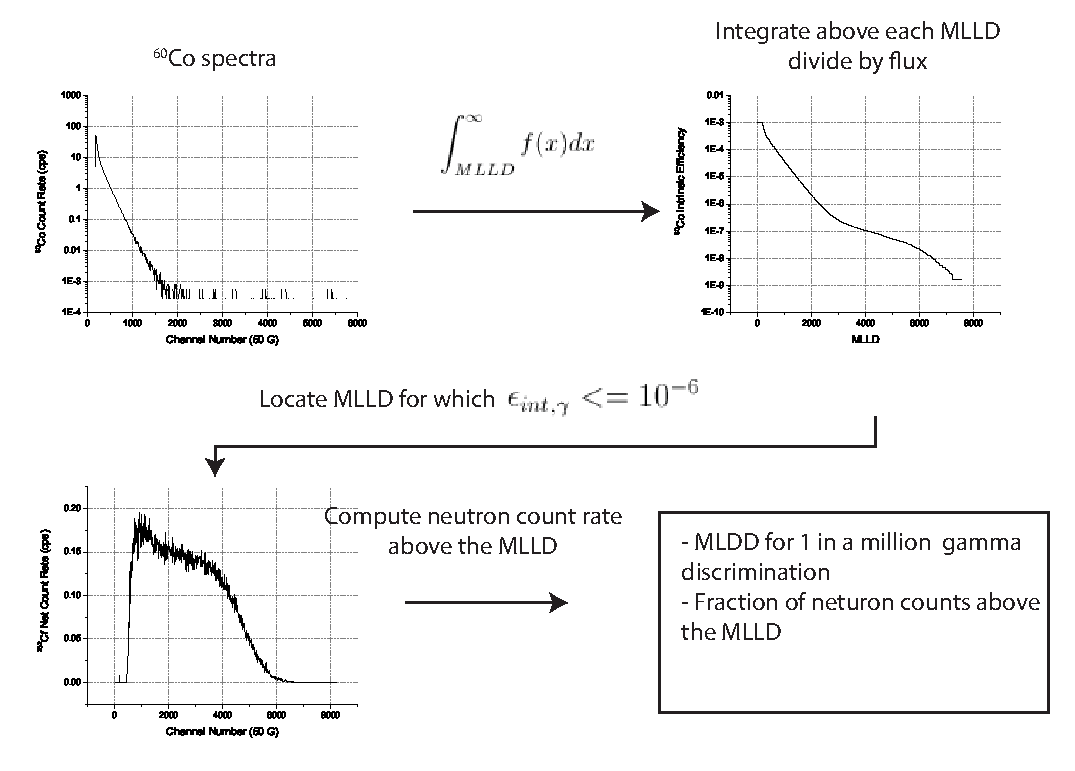
\includegraphics[height=0.5\textheight]{images/CartoonIntEffReal.eps}
		\caption{Determination of the MLLD (Example)}
		\label{fig:ElectronicsPSD}
	\end{figure}
\end{frame}
%%%%%%%%%%%%%%%%%%%%%%%%%%%%%%%%%%%%%%%%%%%%%%%%%%%%%%%%%%%%%%%%%%%%%%%%%%%%%%%
\begin{frame}{Gamma Intrinsic Efficiency Example II}
	\begin{figure}
		\centering
		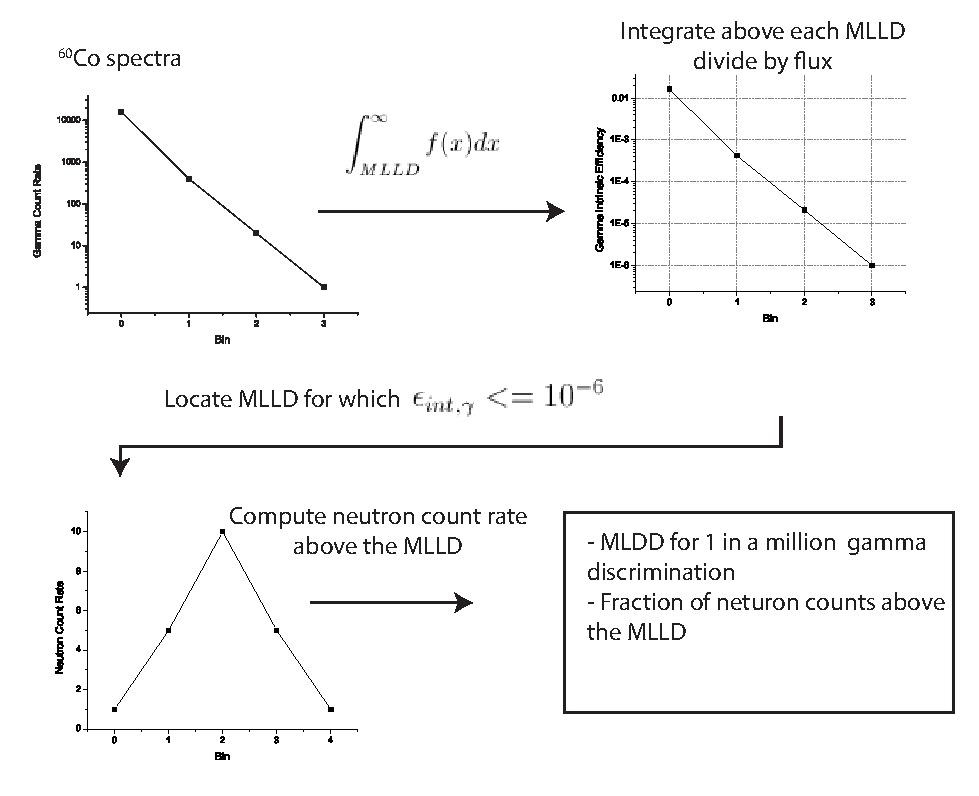
\includegraphics[height=0.5\textheight]{images/CartoonIntEffSimple.eps}
		\caption{Determination of the MLLD for a PEN film}
		\label{fig:CartoonIntEffSimple}
	\end{figure}
\end{frame}
%%%%%%%%%%%%%%%%%%%%%%%%%%%%%%%%%%%%%%%%%%%%%%%%%%%%%%%%%%%%%%%%%%%%%%%%%%%%%%%
%%%%%%%%%%%%%%%%%%%%%%%%%%%%%%%%%%%%%%%%%%%%%%%%%%%%%%%%%%%%%%%%%%%%%%%%%%%%%%%

%%%%%%%%%%%%%%%%
\section{Simulation Validation}
\label{sec:SimValidation}

GEANT4 is a toolkit implemented by the user so extensive efforts were completed in order to validate the results and ensure no bugs exists.
First steps were taken (for small runs) to compute the energy deposition for small runs by hand in order to make sure they agreeded with the analysis code.
In addition the reaction products of the \iso{Li}{6}$(\text{n},\alpha)$\iso{H}{3} were checked to make sure that they agreeded with the published values \footnote{GEANT4 4.9.2.p01 contains an error in which extra photons are generated, \verb+http://hypernews.slac.stanford.edu/HyperNews/geant4/get/phys-list/530.html+. This has been fixed in the release used, 4.9.5p1}.
The GEANT4 simulation was validated by comparing the single collision energy loss spectra in water and by comparing the simulation energy deposition to that of a measured spectra.


\subsection{Energy Deposition Validation}
The energy deposition was tested by reproducing the single collision energy loss spectra in water\footnote{%
An analysis class was not written for this simulation. 
Instead the verbosity of the simulation was set to \verb+verbose=1+ in the run macro.
The first ionisation collision (\verb+e-_G4DNAIonisation+) was then extracted with \verb+sed -n '/ParentID = 0/,/e-_G4DNAIonisation/p' G4OutputFileName.txt+ \verb+grep+ and \verb+awk+ were then used to extract the actual energy, \verb+| grep "e-\_G4DNAIonisatioin" | awk '${print $5}'+ %
}.
The \verb+PhysicsList+ was extended to include \verb+G4DNAPhysics+ and the detector material was set to the NIST definition contained in the toolkit with \verb+G4Material* H20 = man->FindOrBuildMaterial("G4_WATER")+.
In general there was excellent agreement between the simulated energy spectra and a previously published spectra\cite{turner_comparative_1982}.
The simulated spectra had much better resolution at fine energies (corresponding to discrete states) of which Turners did not.
%%%%%%%%%%%%%%%%%%%% Figures %%%%%%%%%%%%%%%%%%%%%%%%
\begin{figure}[h]
    \centering
    \begin{subfigure}[b]{0.45\figurewidth}
        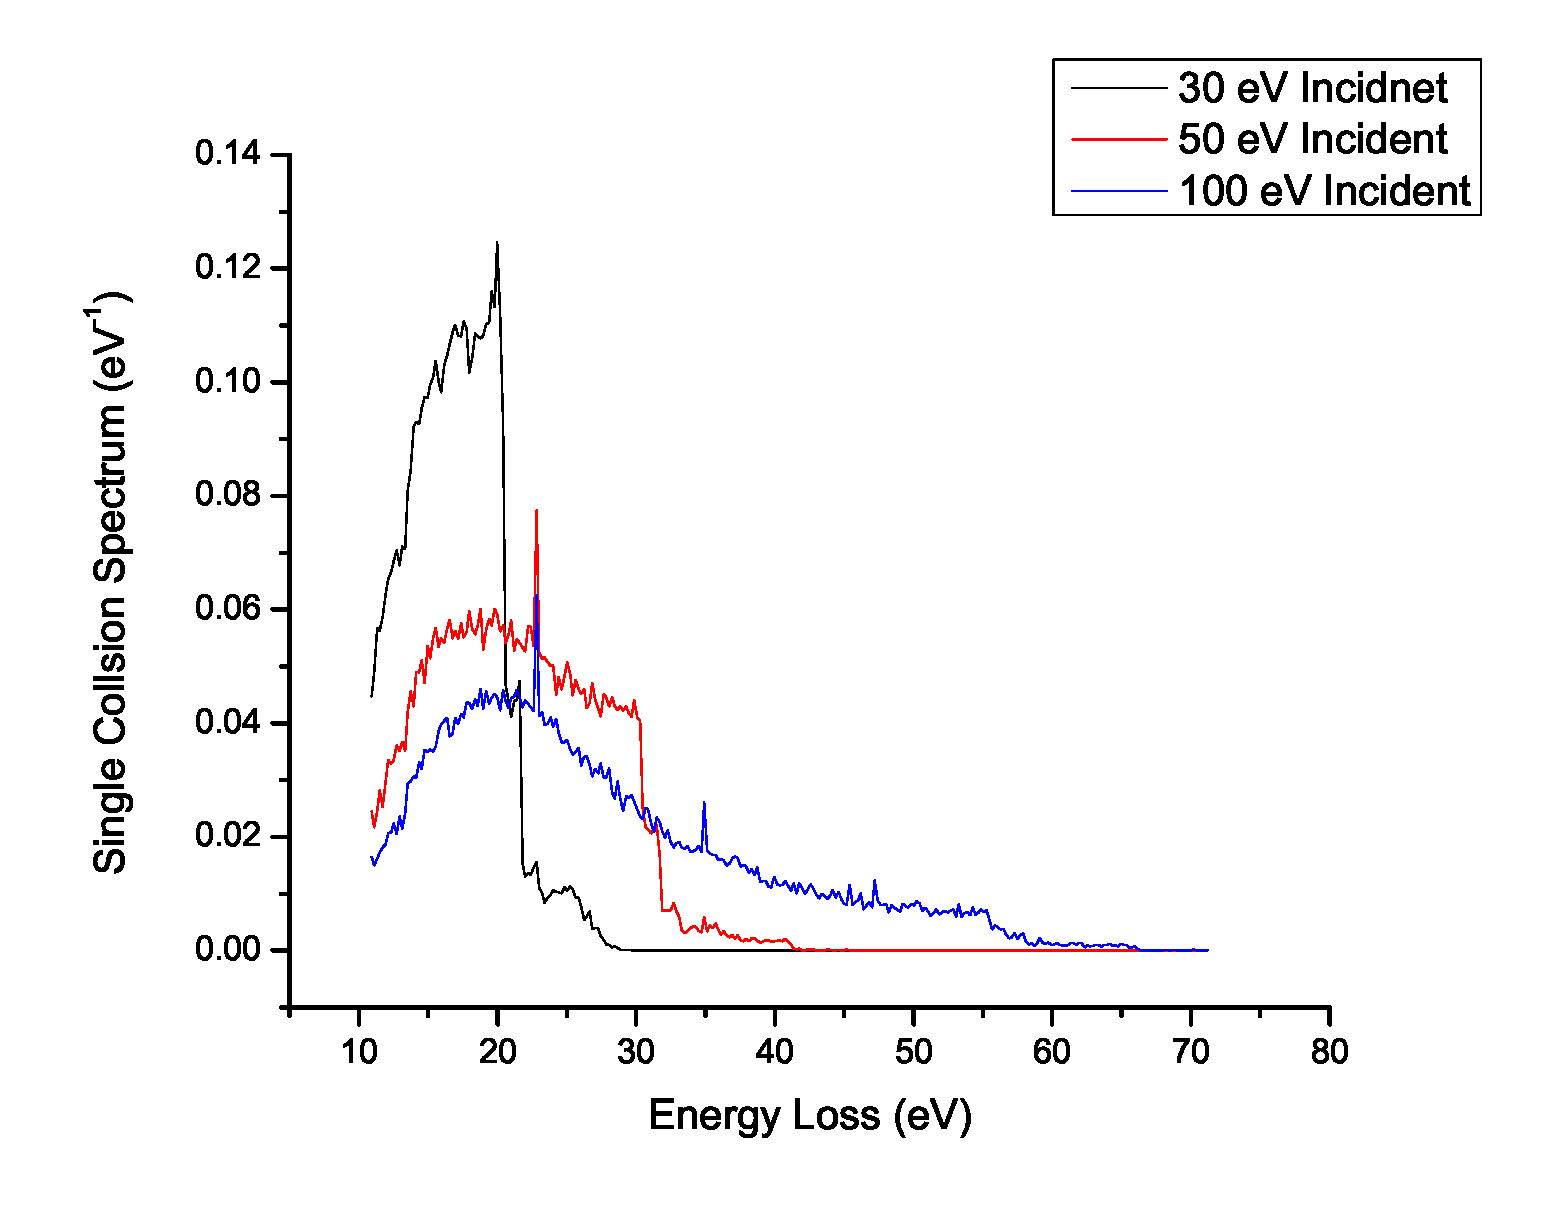
\includegraphics[width=\textwidth]{SingleCollisionEnergyLoss_300bins}
        \caption{Simulated}
    \end{subfigure}
    \begin{subfigure}[b]{0.45\figurewidth}
        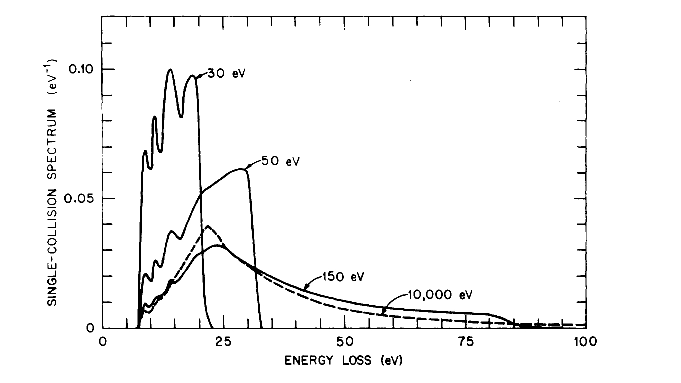
\includegraphics[width=\textwidth]{Turner_Fig2_SingleCollisionELoss}
        \caption{Single-collision energy loss spectra for electrons in water \protect\cite{turner_comparative_1982}}
        \caption{Published}
    \end{subfigure}
    \caption{Single Collision Energy Loss of Water}
\end{figure}
\subsection{Spectra Validation}
The simulated energy deposition is not the directly equivilant to light collected on the PMT because the scintillation process and light collection is not modeled.
However, it is well known that scintillation follows the energy deposition\cite{birks_scintillations_1951}.
Thus, up to scaling contants, the energy deposition can be considered equivilant to the scintillation and representative of the measured spectra.
Rather than attempting to back out these scaling contants the weighted average of spectra were used in which integration and normalization removes these fudge factors.
The simulation was validated by computing the weighted average of the energy deposition \ref{eq:AvgEnergyDepDefination} and comparing it to the spectra average defined in \ref{eq:AvgChannelNumberDefination}.
There is excellent agreement between the measured gamma weighted average (right ordinate axis) and the average energy deposition from a \iso{Co}{60} source (left ordinate axis).
Non-linearity is observed for films less than 200 \micron, this is evidance that the cascade electrons from the Compton electron are eneregetic enough that the range of the electrons is much greater than the thickness of the film and leave the film without colliding to an energy in which the energy deposition is linear (Figure ~\ref{fig:TurnerETransfer}).
%%%%%%%%%%%%%%%%%%%%% Equations %%%%%%%%%%%%%%%%%%%%%%
\begin{equation}
\label{eq:AvgEnergyDepDefination}
<E> = \frac{\int_0^\infty {\phi(E)EdE}}{\int_0^\infty{\phi(E)dE}} \\
\text{where}
\end{equation}
\begin{equation}
\label{eq:AvgChannelNumberDefination}
<\mu> = \frac{\int_0^\infty {f(x)xdx}}{\int_0^\infty{x(x)dx}} \\
\text{where}
\end{equation}
%%%%%%%%%%%%%%%%%%%% Figures %%%%%%%%%%%%%%%%%%%%%%%%
\begin{figure}
    \centering
    \caption{Gamma Simulation Agreement}
    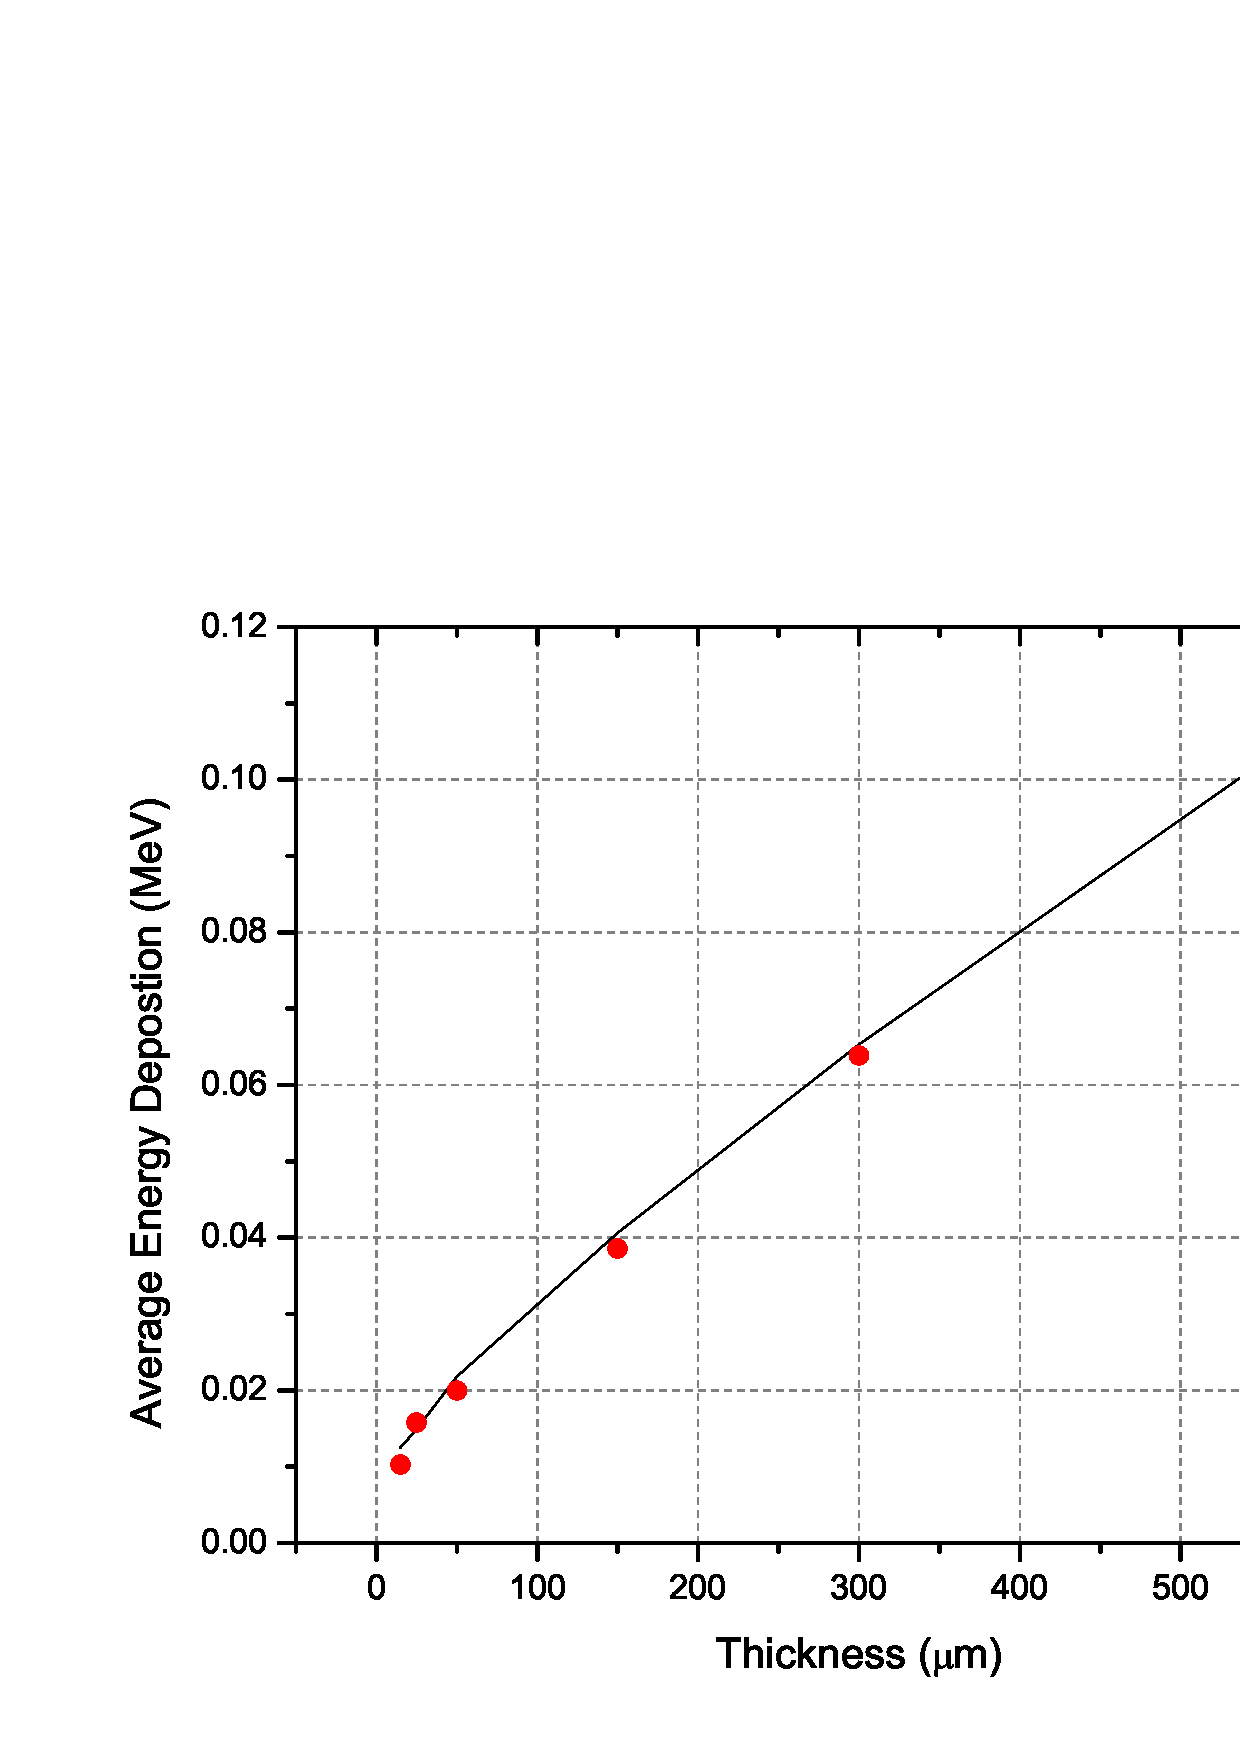
\includegraphics[width=\textwidth]{G4EDep_LightYield_Co60}
    \label{fig:GammaSimAgreement}
\end{figure}
\begin{figure}
    \centering
    \caption{Neutron Simulation Agreement}
    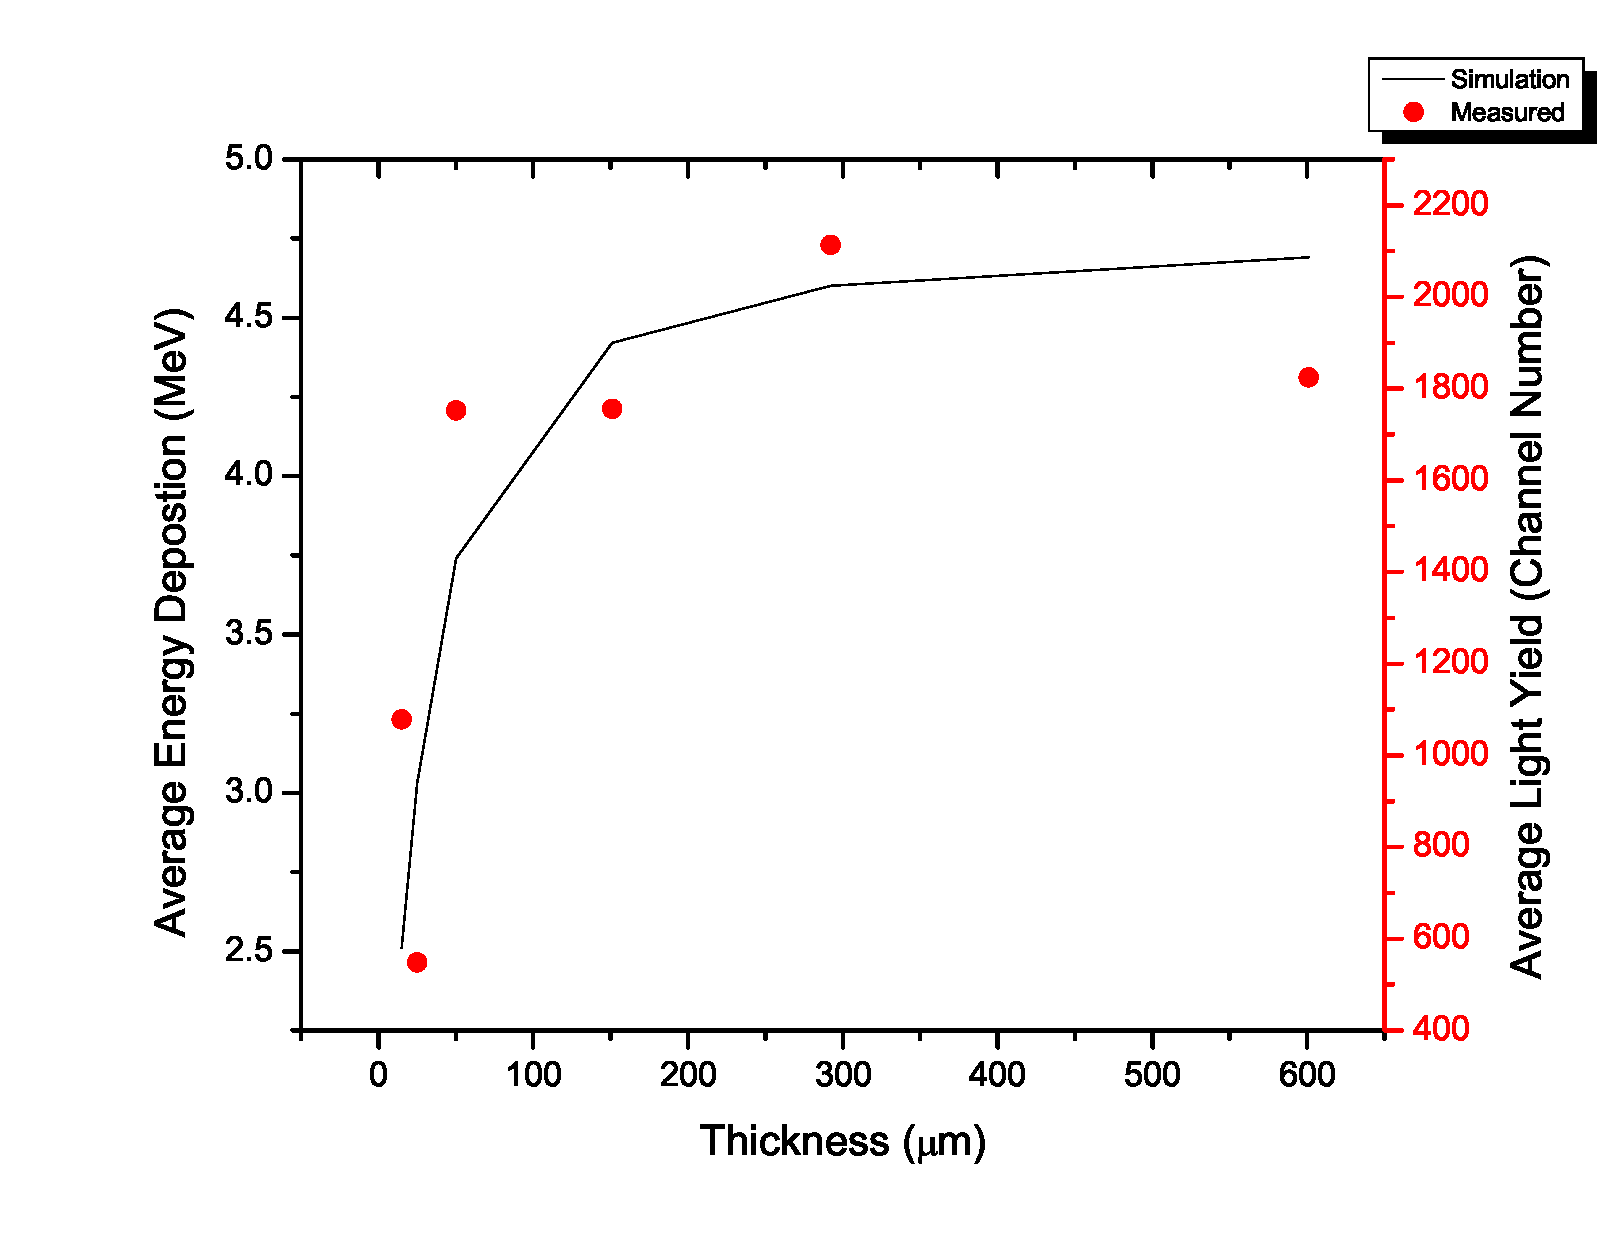
\includegraphics[width=\textwidth]{G4EDep_LightYield_Neutron}
    \label{fig:NeutronSimAgreement}
\end{figure}

The comparison between the average energy deposition and measured channel allows for the a relationship to be drawn between the energy deposited and the channel number.
This is completed by an taking an average of the ratio between the average channel number (Equation \ref{eq:AvgChannelNumberDefination} and the average energy deposition (Equation \ref{eq:AvgEnergyDepDefination}).
This ratio is defined in Equation \ref{eq:ChannelNumber}.  This quantity is defined seperately for neturons and gammas.
%%%%%%%%%%%%%%%%%%%%% Equations %%%%%%%%%%%%%%%%%%%%%%
\begin{equation}
\label{eq:ChannelNumber}
\eta = \sum_t { \frac{<E>}{<\mu}} 
\end{equation}

\section{Results}
\label{sec:Results}

\subsection{Parmater Search}

The parameter search for the optimal C and $\sigma$ parameters is shown in the contour plots of Figures \ref{fig:ParamLiver}, \ref{fig:ParamGlass} and \ref{fig:ParamGlass}.
The optimal classifier parameters are shown for the coarse parameter search in Table \ref{tab:CoarseParamValues} and for the fine parameter search in Table \ref{tab:FineParamValues}.
\todo{Make some quantifications and discuss the data}
\begin{table}[h!]
\caption{Coarse Optimal Classifier Parameters}
\label{tab:CoarseParamValues}
\begin{tabular}{c c c c c c c c}
\hline
Data Set & $C_{min}$ & $C_{max}$ & $\sigma_{min}$ & $\sigma_{max}$ & $C$ & $\sigma$ & $\epsilon$ \\ 
\hline
Glass & 1.00 & 10.00 & -7.00 & 7.00 & 10.00 & 0.37 & 71.67 \\ 
Liver & 1.00 & 10.00 & -7.00 & 7.00 & 10.00 & 0.37 & 74.00 \\ 
Vowel & 1.00 & 10.00 & -7.00 & 7.00 & 10.00 & 1.11 & 99.24 \\ 
\hline
\end{tabular}
\end{table}
\begin{table}[ht]
\caption{Fine Optimal Classifier Parameters}
\label{tab:FineParamValues}
\begin{tabular}{c c c c c c c c}
Data Set & $C_{min}$ & $C_{max}$ & $\sigma_{min}$ & $\sigma_{max}$ & $C$ & $\sigma$ & $\epsilon$ \\ 
\hline
Glass & 5.00 & 15.00 & 0.18 & 0.55 & 14.47 & 0.22 & 74.44 \\ 
Liver & 5.00 & 15.00 & 0.18 & 0.55 & 12.89 & 0.24 & 74.00 \\ 
Vowel & 5.00 & 15.00 & 0.55 & 1.66 & 15.00 & 1.19 & 99.43 \\ 
\hline
\end{tabular}
\end{table}
\begin{figure*}[ht!]
	\centering
	\begin{subfigure}[b]{0.45\textwidth}
		\centering
		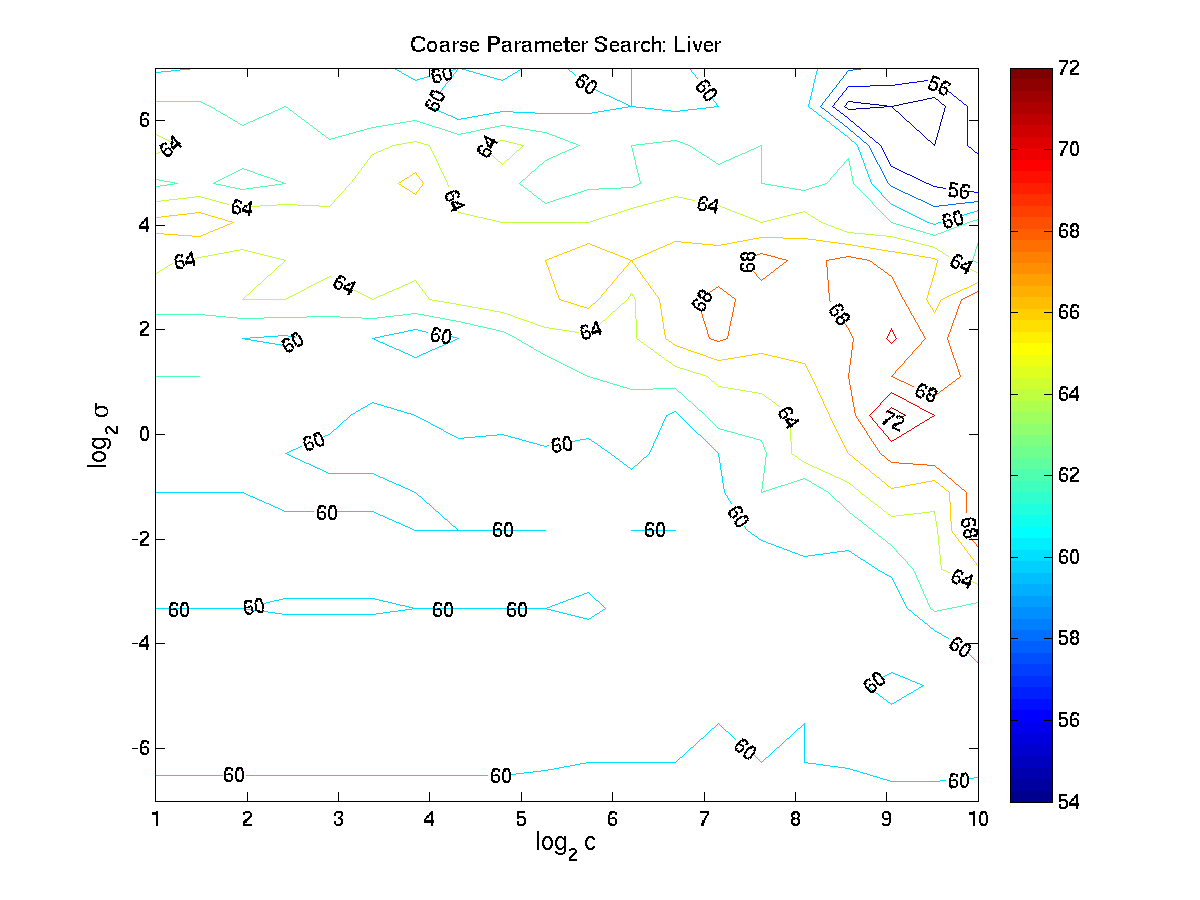
\includegraphics[width=\textwidth]{Liver_coarseSearch}
        \caption{Coarse Search}
	\end{subfigure}%
	~
	\begin{subfigure}[b]{0.45\textwidth}
		\centering
		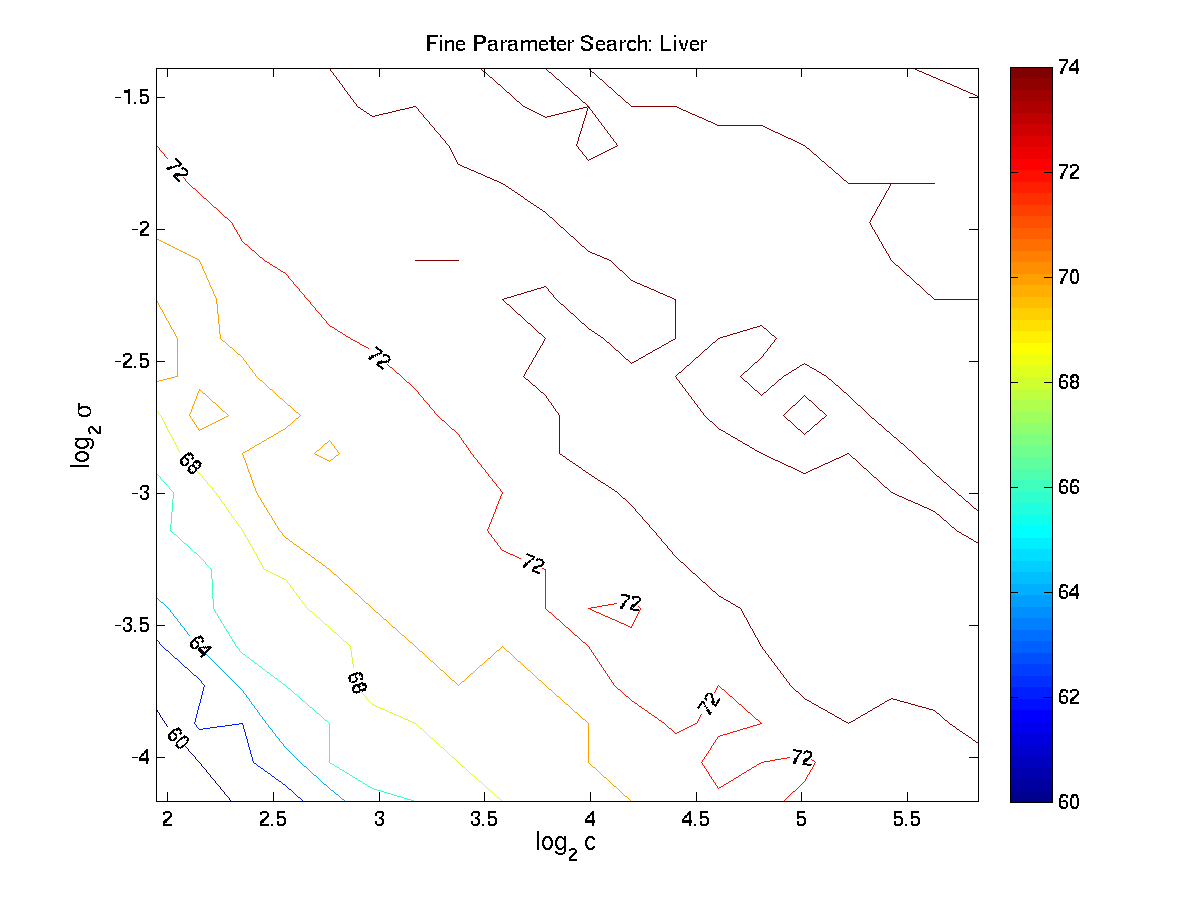
\includegraphics[width=\textwidth]{Liver_fineSearch}
        \caption{Fine Search}
	\end{subfigure}	
	\caption{Parameter search for Liver Disorder}
	\label{fig:ParamLiver}

	\begin{subfigure}[b]{0.45\textwidth}
		\centering
		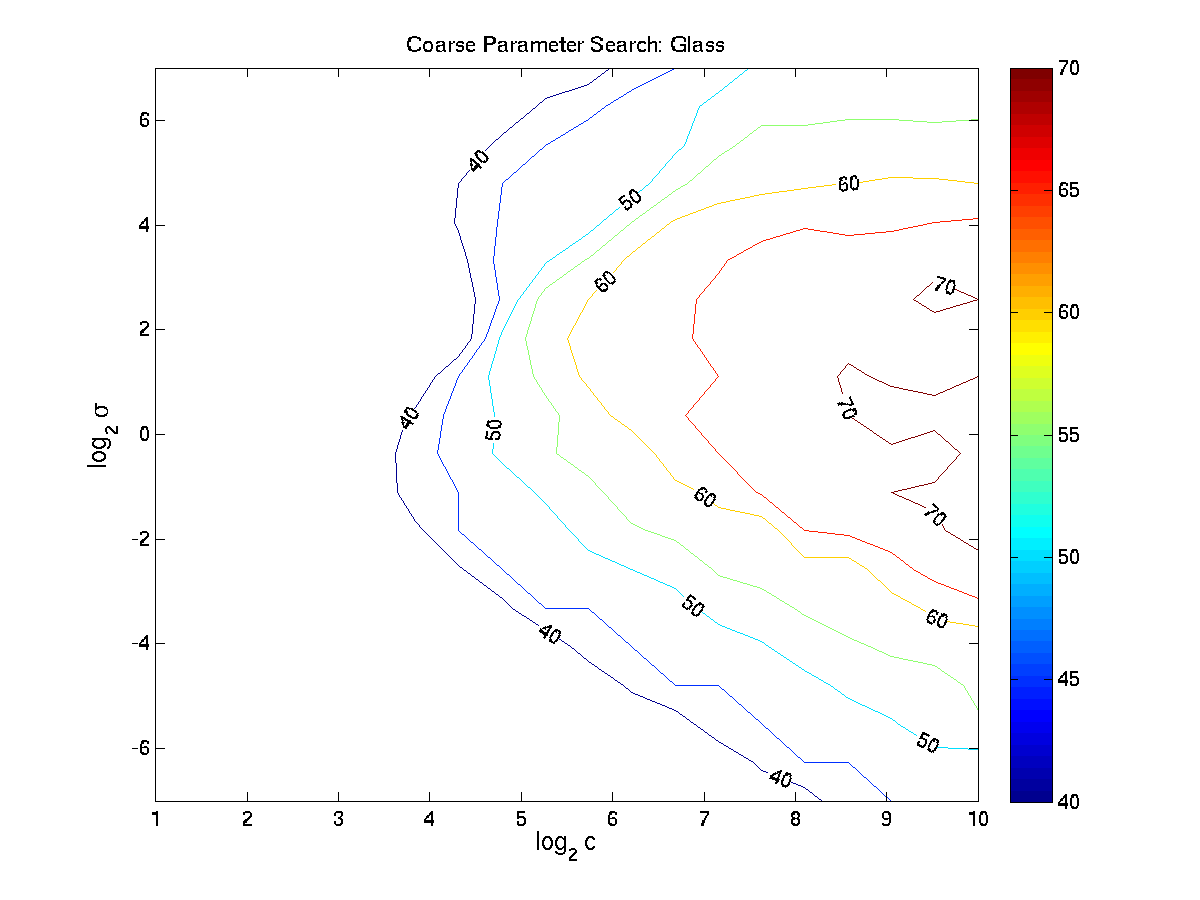
\includegraphics[width=\textwidth]{Glass_coarseSearch}
        \caption{Coarse Search}
	\end{subfigure}%
	~
	\begin{subfigure}[b]{0.45\textwidth}
		\centering
		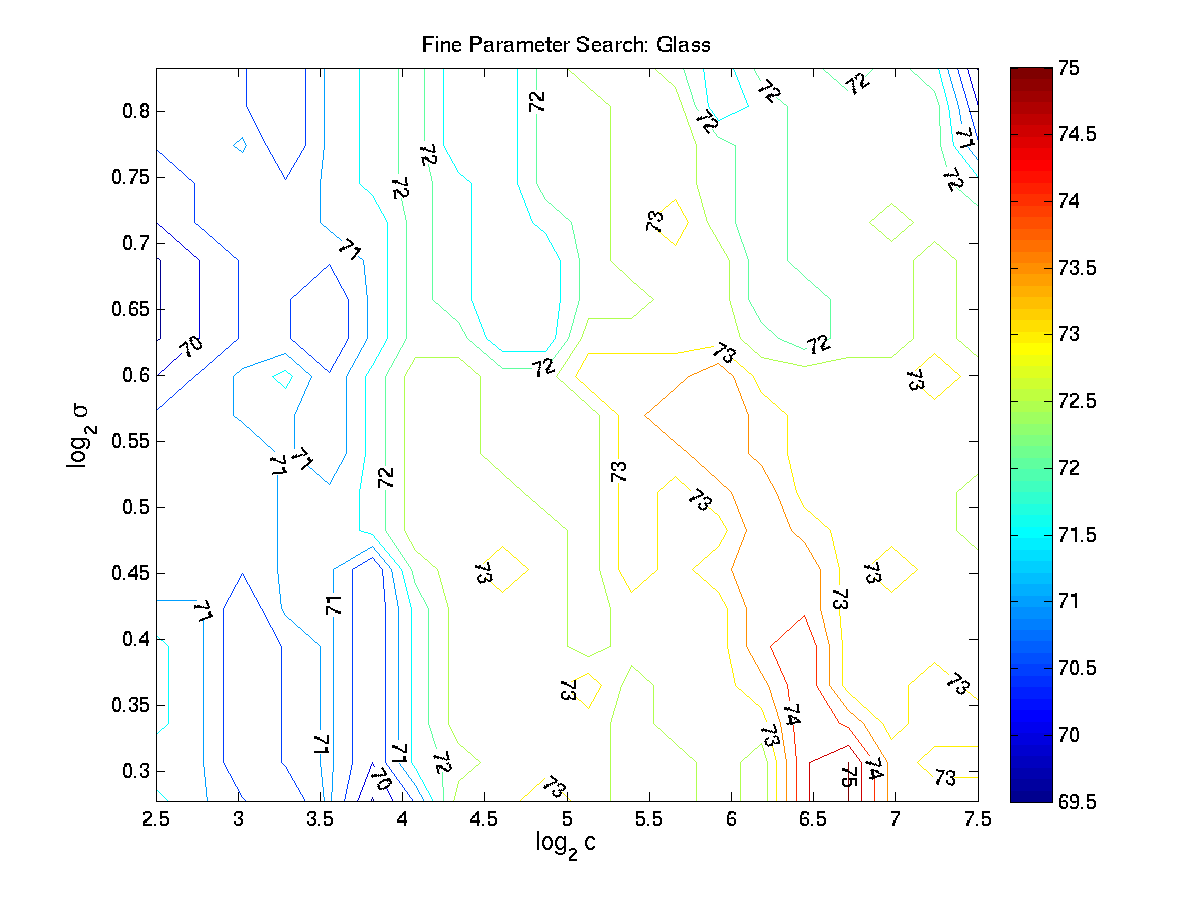
\includegraphics[width=\textwidth]{Glass_fineSearch}
        \caption{Fine Search}
	\end{subfigure}	
	\caption{Parameter search for Glass Disorder}
	\label{fig:ParamGlass}

	\begin{subfigure}[b]{0.45\textwidth}
		\centering
		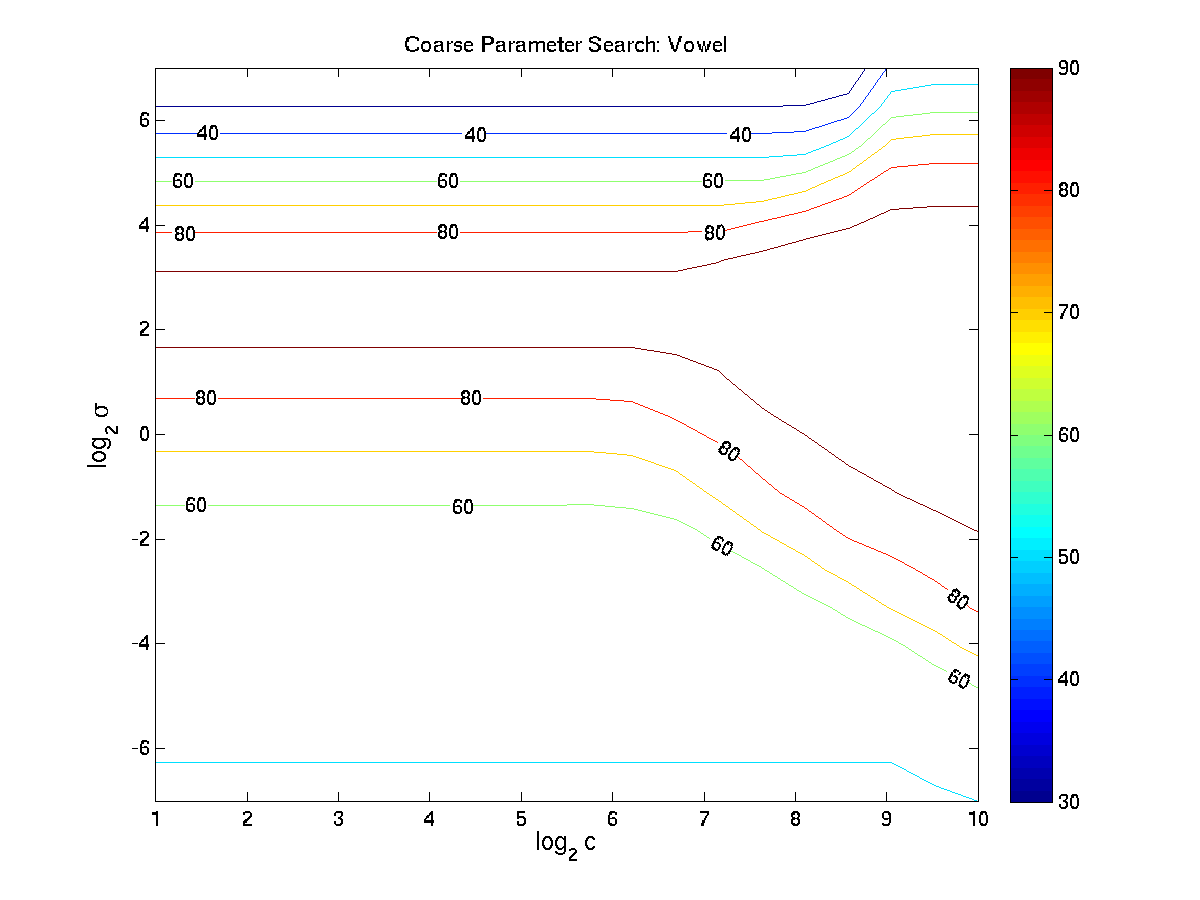
\includegraphics[width=\textwidth]{Vowel_coarseSearch}
        \caption{Coarse Search}
	\end{subfigure}%
	~
	\begin{subfigure}[b]{0.45\textwidth}
		\centering
		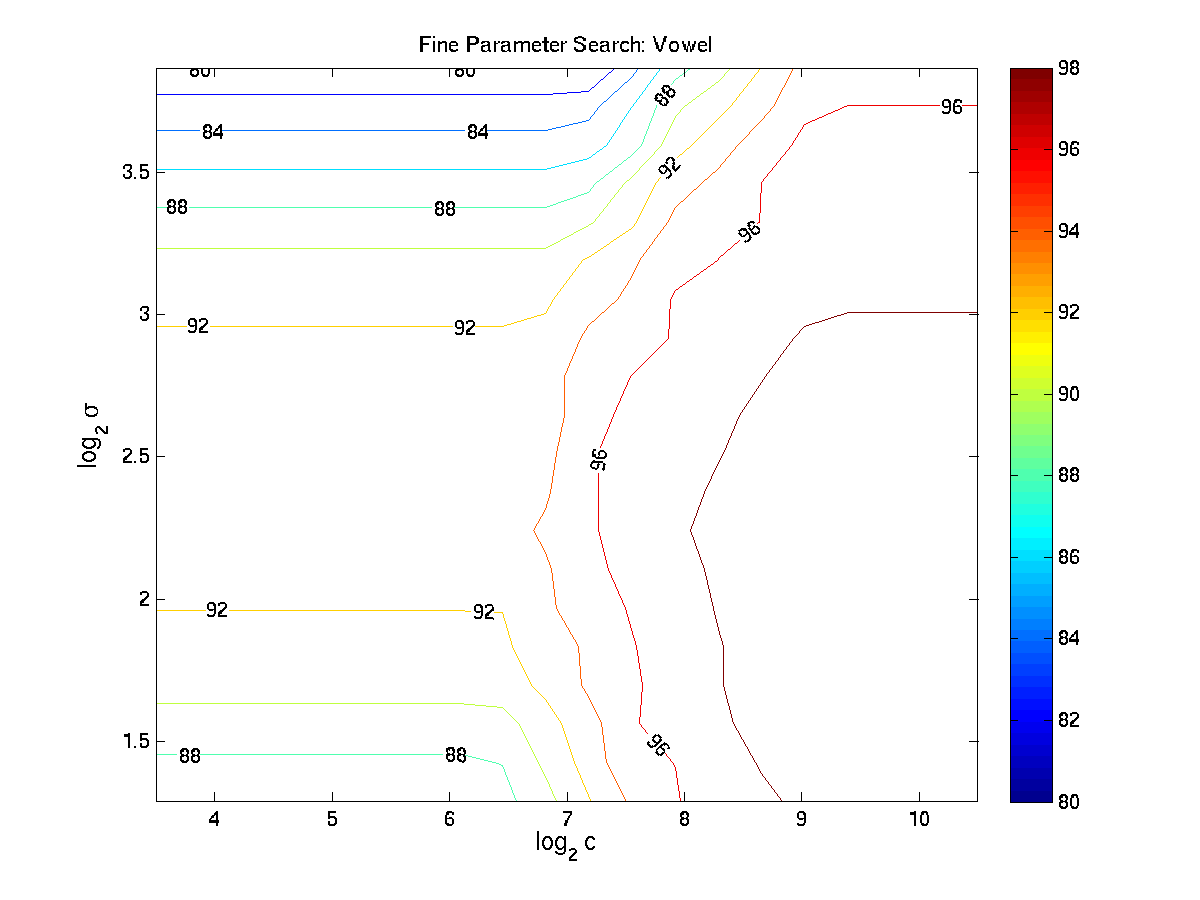
\includegraphics[width=\textwidth]{Vowel_fineSearch}
        \caption{Fine Search}
	\end{subfigure}	
	\caption{Parameter search for Vowel Disorder}
	\label{fig:ParamVowel}
\end{figure*}

\subsection{AdaBoostM1}


% Bibliography
\bibliography{../Zotero}

% Appendix
\appendix
%%%%%%%%%%%%%%%%%%%%%%%%%%%%%%%%%%%%%


\subsection{GEANT4 Implementation}
Visiable light in GEANT4 is known as an optical photon.
An optical photon has momentum ($\vec{p} = \hbar \vec{k}$), corresponding to the energy and direction of the photon, as well as a polarization ($\vec{e}$).
The GEANT4 toolkit breaks up light transport into two parts; the creation of the optical photon an  the tranposrt of the optical photon through the material.
Each of these are material depandent properties which need to be suplied by the user.
This done by creating a material properties table \lstinline{G4MaterialPropertyTable}, of which the following properties are available:
\begin{itemize}
    \item \verb+RINDEX+
    \item \verb+ABSLENGTH+
\end{itemize}
\subsubsection{Scintillation Process}
The number of optical photons generated by GEANT4 is proportional to the energy lost during the step, determing the energy from the emperical emission spectra of the material.
In GEANT4 this is accomplished by creating a \verb+G4Scintillation+ process.\footnote{As the scintilaltion properties are attached to the process and not the material GEANT4 is incapable of more than one scintillation material in any given application.}
\begin{lstlisting}
#include "G4Scintillation.hh"

G4Scintillation* theScintProcess = new G4Scintillation("Scintillation");

theScintProcess->SetTrackSecondariesFirst(true);
theScintProcess->SetScintillationYield(7500.0/MeV);
theScintProcess->SetResolutionScale(1.0);
theScintProcess->SetScintillationTime(45.*ns);
\end{lstlisting}

\subsubsection{Optical Photon Transport}
There are three classes of optical photon interactions in GEANT4:
\begin{itemize}
    \item Refraction and reflection
    \item Bulk Absorption
    \item rayleight scattering
\end{itemize}
Of these only refraction and reflection are necessary. \cite{cern_interactionsOfOpticalPhotons}

\cite{riggi}

\end{document}

